\documentclass[12pt,a4paper]{ctexart}

\usepackage[UTF8]{ctex}
\usepackage{geometry}
\usepackage{graphicx}
\usepackage{xcolor}
\usepackage{tikz}
\usepackage{fontspec}
\usepackage{setspace}
\usepackage{enumitem}
\usepackage{booktabs}
\usepackage{array}
\usepackage{longtable}
\usepackage{hyperref}
\usepackage{fancyhdr}
\usepackage{titlesec}
\usepackage{multicol}
\usepackage{xurl}
\usepackage{tocloft}

\renewcommand{\cfttoctitlefont}{\hfill\bfseries\Large}
\renewcommand{\cftaftertoctitle}{\hfill}
\geometry{left=2.5cm,right=2.5cm,top=2.5cm,bottom=2.5cm}

\definecolor{black}{RGB}{0,0,0}
\definecolor{mainblue}{RGB}{0,82,147}
\definecolor{accentgold}{RGB}{180,140,60}
\definecolor{lightgray}{RGB}{245,245,245}
\definecolor{darkgray}{RGB}{80,80,80}
\definecolor{mainred}{RGB}{230,1,45}

\hypersetup{
    colorlinks=true,
    linkcolor=black,
    urlcolor=mainblue,
    citecolor=mainblue,
    pdfborder={0 0 0}
}

\pagestyle{fancy}
\fancyhf{}
\fancyhead[L]{\small\color{darkgray}\textbf{量子行业每周新闻洞察}}
\fancyhead[R]{\small\color{darkgray}\textbf{总第182期}}
\fancyfoot[C]{\thepage}
\renewcommand{\headrulewidth}{0.4pt}
\renewcommand{\footrulewidth}{0pt}

\titleformat{\section}
    {\Large\bfseries\color{mainred}}
    {\thesection、}{0em}{}
\titleformat{\subsection}
    {\large\bfseries\color{mainred}}
    {\thesubsection、}{0em}{}

\newcolumntype{L}[1]{>{\raggedright\arraybackslash}p{#1}}
\newcolumntype{C}[1]{>{\centering\arraybackslash}p{#1}}

\begin{document}

% ==================== 封面 ====================
\begin{titlepage}
\begin{tikzpicture}[remember picture,overlay]
    \fill[mainred] ([yshift=-0.5cm]current page.north west) rectangle ([yshift=-1.2cm]current page.north east);
    \fill[mainred] ([yshift=1.2cm]current page.south west) rectangle ([yshift=0.5cm]current page.south east);
\end{tikzpicture}

\vspace*{4cm}

\begin{center}
    {\fontsize{44}{52}\selectfont\bfseries\color{black} \textbf{量子行业每周新闻洞察}}

    \vspace{0.8cm}

    {\fontsize{16}{22}\selectfont\color{darkgray} 2026.05.31 — 2026.06.05 }
    {\fontsize{16}{22}\selectfont\color{darkgray} \textbf{WEEKLY NEWS}}

    \vspace{1.5cm}

    {\fontsize{20}{26}\selectfont\color{mainred}\textbf{（总第\textbf{ 182 }期）}}

    \vspace{4cm}

    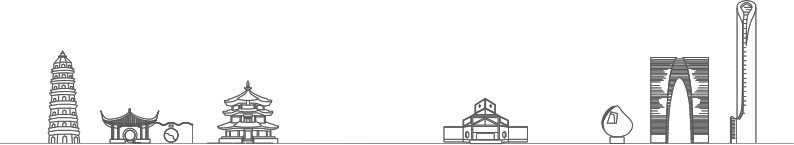
\includegraphics[width=\textwidth]{Cover_Suzhou.png}

    \vfill

    {\fontsize{12}{16}\selectfont\color{darkgray} 量子科技长三角产业创新中心\\编制：战略情报与成果专利室、产业发展部（理事会办公室）}
\end{center}
\end{titlepage}

% ==================== 目录 ====================
\pagenumbering{roman}
\newpage
\tableofcontents

\newpage

% ==================== 摘要 ====================
\pagenumbering{arabic}
\setcounter{page}{1}
\begin{center}
{\Large\bfseries\color{mainred} 摘\hspace{2em}要}
\end{center}
\addcontentsline{toc}{section}{摘要}


\textbf{ 宏观态势：}

全球量子科技正从基础科研向产业应用、人才培养和区域生态构建全面迈进。各国政府与组织纷纷加码布局，如芬兰、欧盟、日本等通过资助项目、成立新机构和制定路线图，系统性地挖掘量子技术在工业、通信和国防等领域的早期应用潜力。同时，高等教育的变革也在加速，多所大学成立量子学院或交叉研究院，旨在储备关键人才。一个显著趋势是，针对量子计算带来的网络安全风险的担忧正在加剧，推动各国开始前瞻性地规划抗量子密码与量子通信基础设施建设，以确保未来的战略自主与数字安全。


\textbf{ 科技前沿：}

量子科技前沿探索呈现多点开花、软硬协同的繁荣态势。底层物理研究持续突破，科学家在宏观量子叠加态材料、新型拓扑磁结构以及利用量子光调控超快激光等领域取得关键进展。面向实用化的工程研发加速推进，多家机构在量子纠错、中性原子编译等核心技术难题上实现里程碑式进展，并设立了清晰的容错计算目标。量子传感领域也展现出巨大潜力，研究者正利用量子精密测量技术探测微弱磁场和运动，相关成果已延伸至生物医学、反潜探测和暗物质搜寻等全新应用场景，跨学科融合趋势显著。


\textbf{ 产品动态：}

量子技术产品化进程显著提速，正从实验室原型迈向专用化解决方案和标准化平台。最引人瞩目的是，包含光量子计算机实现“量子优势”和新型拓扑量子芯片发布在内的重大进展，标志着不同技术路线均向实用化迈出坚实一步。市场涌现出针对特定瓶颈的工具，如突破测量瓶颈的读取技术和面向量子通信的实时威胁检测平台。商业化落地同样深入，量子安全技术正被主动集成到现有AI监控、自动驾驶平台等基础设施中，而云服务和高校专用设备则加速了计算资源的普及，整个生态系统的硬件、软件和安全构件正在快速完善。


\textbf{ 企业资讯：}

尽管本期企业资讯数量有限，但从中仍能洞见量子计算公司战略扩张的两大核心方向。首先，新一轮全球化布局拉开序幕，企业正积极跨越原有地理界限，在亚太等关键市场设立总部，以捕捉更广泛的商业机会。其次，管理团队的迭代升级成为焦点，公司倾向于任命在电信等成熟行业拥有深厚产业化经验的资深人士进入董事会和高管层。这清晰地释放出一个信号：量子技术企业正从纯科研驱动的初创模式，转向由成熟商业领袖掌舵、注重网络操作系统平台化和市场落地的产业化新阶段。


\textbf{ 资本运作：}

本周资本市场用行动证明，量子科技正处于大规模商业化爆发的前夜，融资与投资热度空前。欧洲市场尤为活跃，诞生了该地区量子计算领域迄今为止最大的一笔融资，而多家初创公司也获得超亿欧元级别投资，用于加速硅基、超导等多条硬件路线的商业化。资金不仅流入软硬件开发商，还催生了产业链上游的关键并购与整合，显示出行业成熟度正在提升。同时，政府力量深度介入，以巨额补贴和联合投资的方式支持建立专注于核心制造——如量子晶圆的先进工厂与实验室，标志着资本、产业与政策形成了强大的合力。






% ==================== 会议列表 ====================
{
    \newpage
    \section*{ 6月量子科技行业国内、国际会议}
    \addcontentsline{toc}{section}{ 6月量子科技行业国内、国际会议}
    \scriptsize
    \begin{longtable}{C{0.8cm}L{2.5cm}L{3cm}L{7cm}}
        \toprule[1.5pt]
        \textbf{序号} & \textbf{日期} & \textbf{地点} & \textbf{会议名称} \\
        \midrule
        \endfirsthead
        \toprule
        \textbf{序号} & \textbf{日期} & \textbf{地点} & \textbf{会议名称} \\
        \midrule
        \endhead
        \bottomrule
        \endfoot
        
        1 & 6月1日-3日 & 拉勒米, 美国 & 第四届怀俄明大学量子暑期学校 \\
        \midrule[0.05pt]
        
        2 & 6月1日-5日 & 罗利, 美国 & 2026量子机器学习暑期研讨会 \\
        \midrule[0.05pt]
        
        3 & 6月1日-5日 & 普罗维登斯, 美国 & 第57届APS原子、分子与光物理年会 \\
        \midrule[0.05pt]
        
        4 & 6月2日-4日 & 特隆赫姆, 挪威 & 量子自旋电子学 \\
        \midrule[0.05pt]
        
        5 & 6月3日-4日 & 罗切斯特, 美国 & 量子热力学与退相干 \\
        \midrule[0.05pt]
        
        6 & 6月4日-5日 & 东京, 日本 & Q2B：量子价值路线图 \\
        \midrule[0.05pt]
        
        7 & 6月5日 & 格拉斯哥, 英国 & 量子与社会研究研讨沙盒 \\
        \midrule[0.05pt]
        
        8 & 6月7日-12日 & 圣巴巴拉, 美国 & 第八届国际量子纠错会议 \\
        \midrule[0.05pt]
        
        9 & 6月7日-13日 & 克里特岛, 希腊 & 青年原子光学会议 \\
        \midrule[0.05pt]
        
        10 & 6月8日-11日 & 滑铁卢, 加拿大 & 量子光子学 \\
        \midrule[0.05pt]
        
        11 & 6月8日-20日 & 卡尔热斯, 法国 & 量子技术计算与通信暑期学校 \\
        \midrule[0.05pt]
        
        12 & 6月8日-8月14日 & 洛斯阿拉莫斯, 美国 & 2026洛斯阿拉莫斯量子计算暑期学校 \\
        \midrule[0.05pt]
        
        13 & 6月9日 & 巴黎, 法国 & Q-Day量子风险峰会：后量子密码学与量子密钥分发 \\
        \midrule[0.05pt]
        
        14 & 6月10日-12日 & 华沙, 波兰 & Perspektywy科技女性峰会 \\
        \midrule[0.05pt]
        
        15 & 6月10日-12日 & 多恩比恩, 奥地利 & 第四届砷化镓量子点国际研讨会 \\
        \midrule[0.05pt]
        
        16 & 6月10日-12日 & 埃朗根, 德国 & 神经形态计算前沿 \\
        \midrule[0.05pt]
        
        17 & 6月11日 & 杰克逊维尔, 美国 & 量子当下，医疗未来 \\
        \midrule[0.05pt]
        
        18 & 6月15日-17日 & 苏黎世, 瑞士 & 欧洲集成光学会议（ECIO） \\
        \midrule[0.05pt]
        
        19 & 6月15日-18日 & 格拉斯哥, 英国 & Optica Quantum 2.0会议 \\
        \midrule[0.05pt]
        
        20 & 6月15日-18日 & 赫尔辛基, 芬兰 & 仲夏开放量子系统、退相干及量子-经典交叉会议 \\
        \midrule[0.05pt]
        
        21 & 6月15日-18日 & 洛杉矶, 美国 & 量子器件设计研讨会 \\
        \midrule[0.05pt]
        
        22 & 6月16日 & 巴黎, 法国 & 第5届France Quantum \\
        \midrule[0.05pt]
        
        23 & 6月16日-17日 & 伦敦, 英国 & 第5届年度量子商业化全球大会2026 \\
        \midrule[0.05pt]
        
        24 & 6月16日-17日 & 格拉斯哥, 英国 & Optica 2026量子产业峰会——第5届 \\
        \midrule[0.05pt]
        
        25 & 6月21日-25日 & 塞费尔德, 奥地利 & 第57届欧洲原子系统组年度会议（EGAS 57） \\
        \midrule[0.05pt]
        
        26 & 6月21日-26日 & 塞费尔德, 奥地利 & 第7届塞费尔德量子信息研讨会 \\
        \midrule[0.05pt]
        
        27 & 6月21日-7月4日 & 贝纳斯克, 西班牙 & 量子科学：实现 \\
        \midrule[0.05pt]
        
        28 & 6月22日-24日 & 奥斯陆, 挪威 & IQT北欧：变化世界中的量子技术 \\
        \midrule[0.05pt]
        
        29 & 6月26日 & 汉堡, 德国 & 第7届ISC HPC国际研讨会——监控、可观测性与运营数据分析 \\
        \midrule[0.05pt]
        
        30 & 6月26日 & 汉堡, 德国 & 第2届统一计算中心量子资源研讨会（QRUCH） \\
        \midrule[0.05pt]
        
        31 & 6月26日 & 汉堡, 德国 & 第5届量子及混合量子/经典计算方法研讨会 \\
        \midrule[0.05pt]
        
        32 & 6月26日 & 汉堡, 德国 & 科学与工业数字孪生研讨会——从数据科学家到数据中心 \\
        \midrule[0.05pt]
        
        33 & 6月22日-7月3日 & 雷苏什, 法国 & 2026光子与原子暑期学校：量子气体、光-物质相互作用、量子技术 \\
        \midrule[0.05pt]
        
        34 & 6月23日-24日 & 罗马(纽约州), 美国 & 量子国际年度研讨会（Q4I） \\
        \midrule[0.05pt]
        
        35 & 6月23日-26日 & 阿尔加维, 葡萄牙 & 第3届量子安全网络与系统研讨会（QSNS 2026） \\
        \midrule[0.05pt]
        
        36 & 6月25日-26日 & 波士顿, 美国 & Quantum.Tech World \\
        \midrule[0.05pt]
        
        37 & 6月29日-7月1日 & 汉堡, 德国 & 国际计算科学大会量子计算专题 \\
        \midrule[0.05pt]
        
        38 & 6月29日-7月3日 & 贝桑松, 法国 & 第14届欧洲频率与时间研讨会（EFTS） \\
        \midrule[0.05pt]
        
        39 & 6月29日-7月10日 & 阿斯巴雷拉斯, 西班牙 & La Ricotta暑期学校：干草堆中的量子 \\
        \midrule[0.05pt]
        
        40 & 6月30日-7月1日 & 柏林, 德国 & GITEX欧洲 \\
        \midrule[0.05pt]
        
    \end{longtable}
}




% ==================== 宏观态势 ====================
\newpage
\section{宏观态势}
\vspace{-0.5em}
\noindent\rule{\linewidth}{1.5pt}

\subsection{ 芬兰量子计算研究项目UnloQ获800万欧元资助，将挖掘工业中早期应用场景 }

2026年06月05日消息，由芬兰VTT技术研究中心、赫尔辛基大学和于韦斯屈莱大学联合发起的UnloQ（解锁量子计算优势）项目近日启动，旨在为工业界识别最具影响力的量子计算早期应用场景。该项目并非等待硬件成熟，而是致力于为企业构建切实可行的量子计算应用路径，开发抗噪声软件并开展工业试点项目。项目已获芬兰商务促进局800万欧元资助，归属其“迎接挑战”计划。这笔资金将支持研究人员开展为期五年的长期工作，以帮助芬兰工业在全球量子转型中构建持久竞争优势。

\noindent\textbf{报道链接：}\url{https://www.vttresearch.com/en/project\_news/unloq-project-accelerates-benefits-quantum-computing-industry}

\subsection{ 莱比锡大学加入新成立的欧洲量子学院，以推进欧洲量子技术教育 }

2026年06月05日消息，新近成立的欧洲量子学院（EQA）是欧洲量子技术领域的教育与培训网络，它汇聚了来自欧洲各地的70多家合作机构，其中包括莱比锡大学物理教育方面的科研人员。据介绍，欧洲量子学院旨在构建一个互联互通的欧洲量子技术教育生态系统，覆盖从学校科普、公众推广到本科、硕士、博士课程以及专业职业发展的全链条。

\noindent\textbf{报道链接：}\url{https://www.uni-leipzig.de/en/newsdetail/artikel/advancing-quantum-technology-education-in-europe-leipzig-university-joins-european-quantum-academy-2026-06-01}

\subsection{ Qunova与JHPC-quantum签署备忘录，将免费使用其量子-经典混合平台进行算法研究 }

2026年06月05日消息，韩国量子计算公司Qunova Computing近日与日本高性能计算计划JHPC-quantum签署谅解备忘录，正式成为该国家级计算项目的测试用户计划参与者。JHPC-quantum由日本经济产业省下属NEDO资助，是日本标志性的国家计算计划，其混合平台结合了超级计算机“富岳”与IBM的Quantum System Two，是全球最强大的集成量子-经典计算环境之一。根据备忘录，Qunova将无偿使用该混合平台，并应用其专有的HI-VQE算法攻克量子化学领域最具挑战性的问题。

\noindent\textbf{报道链接：}\url{https://qunovacomputing.com/news/140}

\subsection{ 东湖高新区领导走访调研中科酷原，精准服务助力企业发展 }

6月3日李世庭调研中科酷原。

\noindent\textbf{报道链接：}\url{https://cascoldatom.com/news.php}

\subsection{ 田纳西大学启动K-Quantum计划，以强化区域量子技术领导地位 }

田纳西大学启动K-Quantum，4300万美元州量子倡议，州长Lee参与。

\noindent\textbf{报道链接：}\url{https://news.utk.edu/2026/05/29/ut-launches-knoxville-quantum-accelerator-to-advance-tennessees-future/}

\subsection{ 欧洲航天局启动Saga任务以推动太空量子加密技术战略自主 }

ESA开展Saga天基QKD任务。

\noindent\textbf{报道链接：}\url{https://www.esa.int/Applications/Connectivity\_and\_Secure\_Communications/Wolves\_and\_quantum\_bits\_creating\_the\_Saga\_mission\_patch}

\subsection{ 西安电子科技大学量子科技交叉研究院于日前成立 }

2026年06月02日消息，5月31日，西安电子科技大学举行了量子科技交叉研究院成立仪式。西电是我国电子信息领域科技创新的重要策源地，也是全国第四所获批量子信息科学本科专业的高校，在量子计算、量子芯片等方向有较长时间的研究沉淀。据悉，量子科技交叉研究院将发挥西电电子信息领域的优势，把握量子科技发展这一重大战略机遇，构筑集科研攻关与人才培养于一体的西部量子创新平台和人才高地。

\noindent\textbf{报道链接：}\url{https://phy.xidian.edu.cn/info/1011/11253.htm}

\subsection{ 欧盟量子旗舰计划将于6月启动系列研讨会，聚焦五大路线图 }

2026年06月02日消息，欧盟量子旗舰计划昨日宣布将启动第二轮公开在线研讨会，以支持其《战略研究与产业议程》（SRIA）及相关路线图的更新工作。作为“量子欧洲战略”路线图更新进程的一部分，该研讨会将聚焦于量子通信、量子标准化、量子供应链与赋能技术、量子传感与计量与量子芯片产业化五大路线图，分别于6月12日至29日举行。每场研讨将围绕技术发展、产业视角、战略重点及关键挑战展开深入讨论，为欧洲量子研究、创新与产业化的下一步方向提供参考。

\noindent\textbf{报道链接：}\url{https://qt.eu/news/2026/2026-06-01\_second-round-Community-Workshops-Quantum-Flagship-SRIA-Roadmaps}

\subsection{ 欧盟启动公开咨询以规划欧洲量子通信基础设施EuroQCI的未来 }

2026年06月02日消息，欧盟委员会近日发布了将于未来举办的欧洲量子通信基础设施（EuroQCI）活动的公开咨询，包含六项引导性问题。这项调研为研究人员及专家提供了贡献知识与见解的机会，旨在共同塑造EuroQCI的后续发展方向。收集到的反馈意见将用于指导预计从2027年起由欧盟委员会支持的新一轮EuroQCI活动。公众参与截止日期为2026年6月24日。

\noindent\textbf{报道链接：}\url{https://www.squad-germany.de/en/open-consultation-on-future-euroqci-activities/}

\subsection{ 印度科学研究所IISc与日本Yaqumo在量子技术研发领域签署合作意向书 }

Yaqumo与IISc签署量子合作意向书。

\noindent\textbf{报道链接：}\url{https://yaqumo.com/en/news/311/}

\subsection{ Infleqtion英国量子版图再下一城，牛津创新中心即将投入使用 }

Infleqtion牛津设中心，曾交付英国首台100物理量子比特系统。

\noindent\textbf{报道链接：}\url{https://infleqtion.com/infleqtion-expands-uk-quantum-operations-with-new-oxford-innovation-centre-and-manufacturing-hub/}

\subsection{ 丹麦前科技大使加盟Sparrow Quantum，出任首席商务官一职 }

Sparrow Quantum任命前科技大使Anne Marie Engtoft Meldgaard为CCO。

\noindent\textbf{报道链接：}\url{https://sparrowquantum.com/post/denmarks-outgoing-tech-ambassador-joins-sparrow-quantum-to-help-scale-european-quantum-hardware}

\subsection{ 导航、医疗与科学的变革者：量子传感器如何感知最微弱的运动与磁场 }

量子传感器已用于MEG脑磁图、导航、重力测量等。

\noindent\textbf{报道链接：}\url{https://news.fiu.edu/2026/quantum-sensors-use-atoms-electrons-and-light-as-ultrasteady-rulers-detecting-faint-motion-magnetism-and-gravity-for-navigation-medicine-and-science}

\subsection{ 电控微型非线性光源问世，有望革新量子通信、传感与计算技术 }

2026年06月01日消息，美国埃默里大学领导的研究团队日前开发出一种微型非线性光源，可通过电“旋钮”实现开关或强度调节。研究人员表示，此前从未有人能在如此微小的器件中通过电旋钮调谐二次谐波。整个集成部件宽度仅200纳米出头，比人类头发丝细逾百倍；其中产生的光信号活性区域仅为2至6纳米，比现有大多数二次谐波器件小数十倍，且可控性得到显著提升。相关成果发表在《光学》期刊上，有望为通信、传感和量子计算领域设计更小巧、更灵活的技术提供新路径。

\noindent\textbf{报道链接：}\url{https://news.emory.edu/features/2026/05/esc\_new\_control\_nanoscale\_light\_28-05-2026/index.html}

\subsection{ 大阪大学制备的钴蜂窝状磁性薄膜或催生低成本量子计算技术 }

2026年06月01日消息，日本大阪大学产业科学研究所（SANKEN）的研究人员与合作机构近日在《物理评论材料》上发表一项研究，成功制备出一种特殊薄膜材料，其中钴原子在大范围蜂窝状矩阵内形成局部的蜂窝状排列。这种钴蜂窝结构展现出强烈的磁相互作用，可能对量子计算应用具有重要意义。磁测量结果显示，该化合物在约88K的温度下表现出类似铁磁体的状态。研究人员表示，这一科学突破有望为更低成本的量子计算材料铺平道路。

\noindent\textbf{报道链接：}\url{https://www.sanken.osaka-u.ac.jp/en/achievement/release/20260528.html}

\subsection{ CSIRO与合作者联合发布量子计算赋能能源系统管理路线图 }

2026年06月01日消息，澳大利亚联邦科学与工业研究组织（CSIRO）量子系统团队与国际研究人员合作，在《自然综述·电气工程》上发表了一份路线图，探讨了将前沿量子计算技术与能源系统管理相结合的潜在机遇与挑战。该路线图强调，量子计算有助于解决关键瓶颈，在设备级转换器和系统级电网运控中解锁新的可能性，并识别出可能最早产生价值的领域，包括特定优化问题、高数据量的电网计算、小规模机器学习任务以及系统安全增强等。

\noindent\textbf{报道链接：}\url{https://www.csiro.au/en/news/All/Articles/2026/May/Quantum-computing-could-supercharge-the-energy-transition}

\subsection{ 澳大利亚与国际研究人员合作发表量子计算在能源领域的发展路线图 }

CSIRO发布量子计算用于智能电网路线图。

\noindent\textbf{报道链接：}\url{https://www.csiro.au/en/news/All/Articles/2026/May/Quantum-computing-could-supercharge-the-energy-transition}

\subsection{ Q-CTRL发布白皮书：预计到2027年将为国防物流领域带来量子优势 }

Q-CTRL白皮书：2027年量子国防后勤优势，软件性能提升3000倍。

\noindent\textbf{报道链接：}\url{https://q-ctrl.com/blog/q-ctrl-defines-the-path-to-quantum-battlefield-information-dominance-for-core-military-problems-in-promising-new-outlook}

\subsection{ AISA警告：政府和关键基础设施组织严重低估量子计算带来的网络安全风险 }

2026年05月31日消息，澳大利亚信息安全协会（AISA）近日警告称，政府及关键基础设施组织正低估量子计算技术发展带来的网络安全风险。该协会指出，许多机构需从现在起着手规划向后量子安全的过渡。AISA表示，尽管量子计算带来的威胁看似遥远，但许多组织忽视了确保系统长期安全所需的准备工作，必须识别当前使用中的脆弱加密技术，并规划系统升级路径。该机构称，资产与数据可见性不足仍是主要障碍，从近期多起网络事件看，许多机构对其IT资产和数据缺乏清晰了解，识别需要升级为抗量子加密的部分、制定并执行计划，所需时间可能远超预期。

\noindent\textbf{报道链接：}\url{https://itbrief.com.au/story/australia-warned-over-quantum-cyber-security-risks}

\subsection{ 印度科学研究所成立创新与创业中心，助力量子及深科技初创企业成长 }

2026年05月31日消息，印度科学研究所（IISc）近日在班加罗尔成立了Wadhwani创新与创业中心，旨在助力量子及深科技初创企业成长。该中心同步举办了“2026量子创投节”，为年轻创业者提供了展示量子技术创意的舞台。IISc还推出名为“InQubate”的初创加速器，专注于推动深科技企业发展，目标是通过整合人才、研究与资源，建立强大的生态系统，并连接学术界与产业界。

\noindent\textbf{报道链接：}\url{https://www.newsbytesapp.com/news/science/iisc-opens-wadhwani-centre-to-support-quantum-and-deep-tech-startups/tldr}


% ==================== 科技前沿 ====================
\newpage
\section{科技前沿}
\vspace{-0.5em}
\noindent\rule{\linewidth}{1.5pt}

\subsection{ 神户大学新研究揭示平面霍尔效应在传统材料中也能出现 }

神户大学证明平面霍尔效应三重对称性可在经典材料出现。

\noindent\textbf{报道链接：}\url{https://www.kobe-u.ac.jp/en/news/article/20260602-67841/?utm\_source=EA\&amp;utm\_medium=WEB}

\subsection{ 牛津大学演示一类新型量子叠加态，有望推动量子技术进步 }

2026年06月05日消息，英国牛津大学的研究人员展示了一类新型量子叠加态，其中每个组成部分本身都是高度奇异的量子态。在这项新研究中，该团队演示了一种方法，可以从一系列本身高度非经典的组成中创建叠加态，从而创造出一类新型的“类薛定谔猫态”家族。被引入叠加态的各个组成，包括压缩态、三压缩态或四重压缩态，此前他们已在同一离子阱平台上合成这些态。此次的新突破在于将它们相干地组合成可编程的类薛定谔猫叠加态，并可精确控制每个部分的大小、方向和间距。这一进展拓展了量子计算、量子传感和量子纠错可用的技术手段。相关研究成果已于近日发表在《物理评论X》上。

\noindent\textbf{报道链接：}\url{https://www.physics.ox.ac.uk/news/oxford-physicists-create-new-family-schrodingers-cat-states}

\subsection{ 以色列量子技术公司QXL任命一名知名物理学家为其科学顾问委员会成员 }

2026年06月05日消息，以色列中性原子量子技术公司Quantum X Labs日前宣布，任命魏茨曼科学研究所的Oren Raz教授为其科学顾问委员会成员。Raz教授是以色列知名物理学家，现任魏茨曼科学研究所复杂系统物理系教职，其研究聚焦于从生命到激光的远离热平衡的非平衡物理系统，这一领域对量子计算硬件的实际运行至关重要。

\noindent\textbf{报道链接：}\url{https://investor.quantumxlabs.xyz/pressreleases/detail/f36bc247-7bc6-4c88-a9da-f2888ef4f3b4}

\subsection{ Atom Computing首次在行业内完整展示基于环形码的量子纠错 }

2026年06月05日消息，Atom Computing近日宣布，它首次在行业内完整展示了基于环形码的量子纠错。结果显示，其中性原子系统在计算中使用更多量子比特时，误码率反而会降低。这使得Atom Computing成为了全球仅有的两家展示多轮持续量子纠错的公司之一，也是首次在中性原子平台上实现这一里程碑。据了解，量子纠错是释放量子计算全部潜力的关键。有效纠错的核心要求是，随着系统规模扩大，逻辑量子比特的误码率要随之下降。Atom Computing的该研究成果证明了其中性原子系统满足这一条件，从而加速了迈向实用级量子计算的进程。

\noindent\textbf{报道链接：}\url{https://atom-computing.com/atom-computing-reveals-quantum-error-correction-with-toric-code/}

\subsection{ 芬兰启动Q-GEN项目以探索量子计算与生命科学的融合发展 }

2026年06月05日消息，芬兰近日启动Q-GEN项目，这是一项将量子计算与生命科学相结合的独特研发创新计划，由芬兰国家商务促进局资助，芬兰自然资源研究所牵头，阿尔托大学、芬兰VTT国家技术研究中心及赫尔辛基大学为合作方。该项目旨在利用前所未有的精度、以合乎伦理和安全的方式构建基于生物数据的生物经济。该项目将生命的基本编码DNA与量子计算相结合，为生物数据分析与育种开辟了新可能，而生物信息学正是量子计算极具前景的应用方向，全球相关方法与计算能力正快速发展。

\noindent\textbf{报道链接：}\url{https://www.vttresearch.com/en/project\_news/code-life-and-quantum-computing-come-together-groundbreaking-project-paves-way-next}

\subsection{ 科罗拉多州立大学大学物理学家精确测量助力破解质子半径谜题 }

科罗拉多州立大学测质子半径约0.84飞米，解决半径之谜。

\noindent\textbf{报道链接：}\url{https://natsci.source.colostate.edu/precise-measurement-by-csu-physicists-helps-resolve-long-standing-proton-radius-puzzle/}

\subsection{ 华盛顿大学量子飞跃中心拓展合作版图，联合中西部高校推动科研突破 }

华盛顿大学量子飞跃中心加入中西部量子合作实验室。

\noindent\textbf{报道链接：}\url{https://artsci.washu.edu/ampersand/center-quantum-leaps-grows-its-impact-teaming-midwestern-universities}

\subsection{ 生物量子传感领域新进展：德国研究人员成功通过无线电波操控蛋白质自旋态 }

慕尼黑工业大学发现蛋白质可用无线电波控制自旋量子态。

\noindent\textbf{报道链接：}\url{https://www.tum.de/en/news-and-events/all-news/press-releases/details/proteins-can-be-selectively-controlled-with-radio-waves}

\subsection{ EPFL成为瑞士首个通过自有设施提供量子计算云访问的高校 }

EPFL通过

\noindent\textbf{报道链接：}\url{https://ggba.swiss/en/epfl-offers-cloud-access-to-quantum-computers-for-the-first-time-in-switzerland/}

\subsection{ 通过将量子材料与光耦合，莱斯大学团队为宏观量子纠缠应用开辟新途径 }

2026年06月03日消息，本文内容全由AI翻译，仅供参考
2026年5月29日——量子纠缠是一种粒子相互缠绕的状态。在这种纠缠状态下，一个粒子的特性会影响另一个粒子，即使它们彼此并不靠近。这一现象通常已在仅包含少量粒子的微观量子系统中被观察到，研究人员可以利用它来存储和处理量子信息。莱斯大学教授亓妙（Qimiao Si）感兴趣的是理解并将量子纠缠应用于包含大量粒子的宏观系统中。
在最近发表于《自然通讯》的一篇论文中，亓妙描述了一种方法，该方法不仅能更好地理解量子材料中的量子纠缠，还能使量子纠缠更易于在宏观系统中应用。他的理论认为，可以通过将量子材料与量子光耦合来实现这一点。
“在这一理论中，通过将物质放置在一个小型反射腔中，并推动其接近所谓的量子临界点，我们就可以引入光子，并在光子-物质混合体中诱导出量子纠缠，”亓妙说。他是Harry C. and Olga K. Wiess物理学与天文学教授，也是极端量子材料联盟的主任。
长期以来，制造这种腔光子-物质混合体一直是一个挑战。理论研究表明，为了发生混合，光和物质必须具有非常强的相互作用，而这在工程上很难实现。然而，这一新理论提出，通过使材料接近其量子临界点，可以降低进入这种混合纠缠态的阈值。
“你可以把量子临界点看作一个材料可以在两个不同量子相之间‘选择’的点，”莱斯大学研究生、该研究共同第一作者王翊铭（Yiming Wang）说。“材料处于一个相中。只有达到量子临界点，它才能转变到第二个相。”
在这一新理论中，研究人员可以通过非热方法（例如施加压力或用一种化学成分替换另一种）来放大光与物质的纠缠，而无需依赖热量，而是依靠物质接近量子临界点的强制近距条件。材料越接近其量子临界点，强量子纠缠的阈值就越低。如果在材料接近量子临界点时将光引入反射腔，那么将两者纠缠起来应该会大大更容易。
“一旦光和物质发生纠缠，它们的各自特性就会相互反映，”莱斯大学前博士后研究员、该论文共同第一作者Shouvik Sur说。“如果材料在与光纠缠的状态下进入量子临界点并转变到第二个相，光也会随之转变。”
因此，实验物理学家可以利用这种方法不仅实现光与物质的纠缠，还可以利用现有针对光和物质的各种方法，在不同相中研究纠缠粒子。这还为研究人员提供了一种方式，在下一代量子技术中利用量子纠缠。
去年，亓妙的研究小组发现，在被称为奇异金属的量子临界材料中，量子纠缠不仅存在，而且被增强。这种量子纠缠可能是量子技术的重要资源——如果科学家能够弄清楚如何从中提取它的话。这一新理论允许利用量子光来提取量子纠缠：在光子和物质发生纠缠后，光可以从腔中提取出来。这样的系统可能有助于开发量子传感等下一代技术。
“最终，这揭示了利用量子光从物质中获取量子纠缠的一条路径，”亓妙说。“这可以为提取量子纠缠资源以及从量子材料中实现新功能奠定基础。”
这项研究得到了美国能源部科学办公室基础能源科学计划（DE-SC0026179）、空军科研办公室（FA9550-21-1-0356）、Robert A. Welch基金会（C-1411）以及Vannever Bush教师奖学金（ONR-VB N00014-23-1-2870）的资助。

\noindent\textbf{报道链接：}\url{https://news.rice.edu/news/2026/rice-physicists-advance-ways-retrieve-matters-quantum-entanglement}

\subsection{ Zapata Quantum任命新产品与市场高管，加速量子计算商业化进程 }

2026年06月03日消息，本文内容全由AI翻译，仅供参考
2026年6月2日——量子计算算法与应用开发领域的领导者Zapata Quantum今日宣布任命Jhonathan Romero Fontalvo博士为产品副总裁，Ian Rotondi-Gray为合作伙伴关系与市场战略高级总监，此举将进一步强化公司的产品开发与商业执行能力。
“量子领域正迎来激动人心的时刻，成功的关键将取决于将技术突破转化为变革性商业成果的能力，”Zapata Quantum首席执行官Sumit Kapur表示。“这些任命加强了对这一课题的两方面支撑——深厚的产品领导力和企业执行力——并使Zapata能够加速客户采纳与长期增长。”
量子与AI先驱Romero Fontalvo博士出任产品副总裁
Romero Fontalvo博士是Zapata的原始联合创始人之一，在Axiomatic AI任职后回归，他曾致力于推动自主式AI在科学发现中的应用。作为产品副总裁，他将专注于开发工具，使量子应用的发现、开发和部署更加系统化和可规模化。
在联合创立Zapata之前，他是哈佛大学变分量子算法（VQAs）的先驱之一。VQAs是行业最早期的验证点之一，促成了对实用量子计算的初步探索。他还曾担任DARPA量子基准测试计划的联合首席研究员，直接与企业客户合作，将实际问题映射为可行的量子解决方案。
“在量子领域，知道哪些应用应优先处理、何时能发挥作用以及如何开发它们，是一个被低估的挑战——我们在与DARPA、BP及其他机构的合作中亲身感受到了这一点，”Romero表示。“我很兴奋能够打造新一代工具来回答这些问题，利用量子算法和人工智能的进步，大幅加速具有商业意义的量子应用的发现与开发。”
企业软件资深人士Rotondi-Gray出任市场战略负责人
Ian Rotondi-Gray加入Zapata之前，曾在Palantir和Oracle担任推动先进技术商业应用的职务。他拥有将新兴技术与客户需求和商业成果相结合的丰富经验。作为市场战略负责人，他将专注于加快Zapata的Quantum Application Intelligence™平台的采纳，并拓展公司的商业覆盖范围。
“吸引我加入Zapata的是公司在高价值领域建立起来的信誉和影响力基础，”Rotondi-Gray表示。“从与DARPA和财富500强企业的合作，到其领先的量子药物发现研究被《自然生物技术》评为2025年十大论文之一，Zapata积累的成就是量子领域（尤其是软件方面）很少有公司能比拟的。我很兴奋能够在此基础上继续推进领导力，并扩大量子应用的商业采纳和实际影响力。”

\noindent\textbf{报道链接：}\url{https://investors.zapataquantum.com/news-releases/news-release-details/zapata-strengthens-product-and-commercial-leadership-quantum}

\subsection{ Quantinuum与三菱电机将联手探索量子计算在先进工程领域的应用前景 }

2026年06月03日消息，量子计算公司Quantinuum昨日与三菱电机签署了一份不具法律约束力的谅解备忘录，双方将建立战略合作框架，共同推动量子计算在先进工业工程与设计领域的应用开发。该合作将聚焦于识别高影响力的工业应用场景，探索量子及量子-经典混合方法，以支持下一代工程工作流程。初步关注领域包括计算机辅助工程（如计算流体动力学），以及利用Quantinuum量子平台上的逻辑量子比特操作进行更广泛的仿真与设计应用。

\noindent\textbf{报道链接：}\url{https://www.quantinuum.com/press-releases/quantinuum-signs-mou-with-mitsubishi-electric-to-launch-strategic-quantum-computing-partnership}

\subsection{ 神户大学新研究利用更精细的数学来区分量子材料与传统材料 }

2026年06月03日消息，神户大学的一个研究团队近日在《物理评论B》上发表新论文，重新审视了平面霍尔效应作为探测特殊量子性质工具的可靠性。该团队通过更精细的数学分析发现，传统材料的三重对称性其实也能产生与量子材料相似的电压模式。此前在经典材料实验中观测到的特殊信号，正是由于这些未被充分考虑的数学细节所致。该研究表明，通过破译电子流动的隐藏规律，可从宏观电学测量中提取微观晶体对称性和电子结构的信息。

\noindent\textbf{报道链接：}\url{https://www.kobe-u.ac.jp/en/news/article/20260602-67841/?utm\_source=EA\&utm\_medium=WEB}

\subsection{ 英日科学家开发出新型光频超精密测量技术，精准度提升34倍 }

2026年06月03日消息，英国牛津大学、伦敦帝国理工学院与日本冲绳科学技术大学院大学的研究团队最近展示了一种新型光频超精密测量技术，可分辨传统光谱学无法企及的微小频率差异。在测试由两条极窄光谱线组成的信号时，该技术成功分辨出仅为信号线宽二十分之一的频率间隔——即在5.3兆赫宽的信号中区分出了265千赫的差异。与标准直接探测方法相比，该技术将测量精度提升了最高34倍。相关研究成果已于日前发表在《自然·传感器》上。

\noindent\textbf{报道链接：}\url{https://www.physics.ox.ac.uk/news/quantum-memory-sharpens-precision-measurements}

\subsection{ 德国启动旨在利用集成光子学与量子通信技术增强光纤网络安全的新合作项目 }

2026年06月03日消息，近日，德国图林根州批准了一项为期三年的合作项目“单光子处理与光子集成偏振分析模块（PIC-PAM）”，项目由欧盟共同资助。该项目将紧密整合图林根州在光学与光子学、微电子及传感器技术领域的优势，其核心目标是通过结合集成光子学与量子通信，实现重大创新突破，以增强德国ICT光纤网络的网络安全。项目合作伙伴包括Quantum Optics Jena、弗劳恩霍夫应用光学与精密工程研究所（IOF）等多家单位。

\noindent\textbf{报道链接：}\url{https://www.iof.fraunhofer.de/en/pressrelease/2026/PIC-PAM.html}

\subsection{ QScale量子项目获芬兰政府资助，将探索光学控制实现超精确信号处理 }

2026年06月03日消息，本文内容全由AI翻译，仅供参考
2026年6月2日——由芬兰国家技术研究中心（VTT）协调、坦佩雷大学和阿尔托大学共同参与的QScale联合项目，已获得芬兰国家商业促进局著名“挑战计划”的资助。在该项目中，研究人员正致力于通过光学控制及基于量子现象的超精确信号技术，从根本上提升量子计算机的能效和可扩展性。量子技术要实现在社会重大影响领域的应用突破，仍需要像QScale这样的重大研究项目铺路。
理论上，量子计算机能够完成经典计算机无法实现的运算。因此，人们期望它们能在化学、生物科学和人工智能等领域带来突破。超导量子计算机是最有前景的技术路径之一，对芬兰而言也是国家层面最重要的方向。
量子计算机的产业化开发进展迅速，但现有技术在扩展到超过1000个量子比特时就会遇到困难，而当目标是一百万个量子比特时则变得不可能。然而，这恰恰是实现量子计算承诺所需的规模。按照现有技术，这样一台量子计算机的能耗将堪比整个核反应堆的发电量，使其在实际上无法实现。
QScale：将光学控制与精确信号技术相结合
QScale项目的主要目标是开发一种芬兰发明的全新方法，用于扩展量子计算机及其他量子技术的规模。该项目将超快、高能效的光通信技术与超导电路相结合，后者能产生近乎完美、无噪声的电信号，为敏感的量子技术带来了巨大优势。
光通信技术还有助于无缝连接量子计算机和超级计算机的计算能力，这预计将使人工智能计算更加高效。
从研究迈向新的商业应用
该项目的目标是到2030年代实现技术商业化，首先用于控制超导量子计算机，随后扩展到众多其他应用。
这个跨学科项目将集成光学、光电子学、半导体电子学和超导电子学与新型电冷却方法相结合。基于芯片的可扩展解决方案将被封装成紧凑模块，这可能开启低温技术的新纪元。此外，研究人员将使终端用户能够方便地获取超精确电信号。其目标是引发电子学领域的一场变革，类似于原子钟曾在基于精确时间和频率的应用中催生的变革。
为期三年的QScale项目将于2026年9月1日启动，总预算约为690万欧元。芬兰国家商业促进局提供的资助金额为550万欧元。

\noindent\textbf{报道链接：}\url{https://www.vttresearch.com/en/news-and-ideas/qscale-new-signal-technology-being-developed-finland-scale-quantum-applications}

\subsection{ D-Wave发布门模型量子计算路线图，2032年实现100逻辑量子比特系统 }

2026年06月03日消息，D-Wave Quantum近日发布了全新的门模型路线图，以加速开发商用级容错量子计算。该公司表示，它将利用其在高相干双轨量子比特和量子纠错方面的专长，并结合其在超导量子系统工程化、规模化及商业化方面的成熟能力来推进这一计划。路线图列出了具体的里程碑节点：2026年交付一个17物理量子比特的系统，使逻辑错误率低于物理错误率2倍；2027年完成49个物理量子比特系统，能实现错误率降低20倍；2028年完成181物理量子比特系统，实现错误率降低2000倍；2030年完成10逻辑量子比特系统，能支持首批容错算法；2032年完成100逻辑量子比特系统，可支持超过100万次操作。

\noindent\textbf{报道链接：}\url{https://www.dwavequantum.com/company/newsroom/press-release/d-wave-charts-a-new-course-to-fault-tolerant-quantum-computing-with-gate-model-roadmap/}

\subsection{ 五年百亿：IBM斥巨资欲加速量子计算突破，目标2029年实现大规模容错计算 }

2026年06月03日消息，本文内容全由AI翻译，仅供参考
2026年6月2日——IBM 宣布计划在未来五年内向量子计算领域投资超过 100 亿美元。这项投资将涵盖研发、资本支出、制造规模扩大、生态系统合作伙伴关系以及并购。这些领域共同旨在加速 IBM 的量子路线图，超越其在 2029 年交付全球首个大规模、容错量子计算机的目标，并巩固其以美国为中心的量子领导地位。
该投资建立在业界最广泛的量子基础之上，包括全球规模最大的量子计算机集群、使用最广泛的量子软件，以及一个由 340 多个组织组成的、正在运行实际工作负载的客户与合作伙伴网络。这项投资将为这一基础的下一阶段提供资金，将 IBM 的领先地位从当今的商业量子计算机推向容错规模系统。
“量子时代已不再遥不可及，它已经开启。我们全球的客户、合作伙伴和用户正在利用 IBM 量子计算机完成几年前不可能完成的工作，”IBM 董事长兼首席执行官 Arvind Krishna 表示。“量子计算机的发现速度正在迅速加快，这项投资将增强我们交付下一代量子硬件、软件和制造能力的能力。”
IBM 当前的量子领导地位
这项投资强化了 IBM 将实用量子计算带给世界的使命，并建立在业界最先进的量子项目基础之上：
庞大的全球量子机队：IBM 运营着全球规模最大、功能最强大的量子计算机集群。截至目前，该公司已通过云和专用现场部署在全球部署了超过 90 套量子系统——其数量超过业界其他公司的总和。这支机队包括在纽约州和德国的 IBM 量子中心、俄亥俄州的克利夫兰诊所、纽约州的伦斯勒理工学院、魁北克的 PINQ、东京大学和日本理化学研究所、韩国延世大学、西班牙 BasQ 运营的量子计算机，并即将在芝加哥和印度阿马拉瓦蒂量子谷增加新系统。
全球首个大规模容错量子计算机路线图：IBM 有明确的路径，计划于 2029 年交付 IBM Quantum Starling——全球首台大规模容错量子计算机，其可执行的操作次数将比现有系统多 20,000 倍。Starling 将为 IBM Quantum Blue Jay 奠定基础，后者将跨 2,000 个量子比特执行 10 亿次量子操作。这些系统将提供转型所需的规模，使量子计算能够解决科学和工业领域中最具挑战性、目前最棘手的问题。
采用范围不断扩大：自 2017 年以来，IBM 的量子项目已与客户签署了超过 11 亿美元的合同，以推进他们对量子计算的探索和使用。如今，一个由 340 多个 IBM 量子网络成员组成的网络——涵盖金融服务、医疗保健、材料科学、学术界和政府——正在使用 IBM 量子计算机进行现实世界中的算法发现。
美国首个量子代工厂：在美国商务部的支持下，IBM 最近宣布计划推出 Anderon，这是全球首家纯量子晶圆代工厂。IBM 将向 Anderon 投入 10 亿美元现金，并附带大量知识产权、资产和一支熟练的劳动力队伍。
通向量子优势之路：IBM 确信，其使用 IBM 量子计算机的合作伙伴将在 2026 年展示量子优势。该公司看到这条道路上的进展正在加速，最近的实验证实了量子计算作为一种有用科学工具的价值，包括与克利夫兰诊所和日本理化学研究所合作对 12,635 个原子的蛋白质进行建模；与国家级实验室和大学合作精确模拟磁性材料；以及与大学合作证明一种前所未见分子的性质的研究。
全球最受欢迎的量子软件：由 IBM 开发的 Qiskit 是全球首选的量子计算和算法研究软件堆栈，旨在优化和执行量子工作负载，目前近 70\% 的量子开发者在使用它，并且已经在量子计算机上执行了超过 4 万亿个量子电路。

\noindent\textbf{报道链接：}\url{https://newsroom.ibm.com/2026-06-02-ibm-commits-more-than-10-billion-to-quantum-computing,-funding-its-roadmap-from-todays-leading-systems-to-the-worlds-first-fault-tolerant-quantum-computers}

\subsection{ 科学家通过精细调控纳米粒子结构，实现了一种仅理论预测过的材料相 }

2026年06月02日消息，来自布朗大学和密歇根大学工程学院的研究人员，通过精细调控一种纳米级构建块，成功稳定了一种理论上被预测但此前从未在物理材料中实现的物质结构相。该团队利用这种银纳米粒子超晶格结构，在室温下重现了Nishiyama-Wassermann路径中那些因对称性低而稍纵即逝的过渡相。该结构不仅能揭示这种相变的新细节，还展现出非凡的光学特性，有望用于量子计算或其他量子信息系统。相关研究成功以在《科学》杂志上发表。

\noindent\textbf{报道链接：}\url{https://www.brown.edu/news/2026-05-28/superlattice}

\subsection{ 荷兰科学家正开发一种高灵敏度传感器，以探测海上难以追踪的“黑船” }

2026年06月02日消息，由荷兰阿姆斯特丹应用科学大学牵头的一个研究团队正致力于开发新一代高灵敏度传感器系统，以探测海上那些不发射识别信号、意图不轨且难以追踪的“黑船”。该项目融合了光子学、光学系统与量子技术，旨在提升海上态势感知能力并强化安全保障。该技术依托先进光学与光子传感器，能够高精度测量极微弱信号。据悉，项目旨在提高在恶劣天气、低能见度等复杂海洋环境下的探测精度。除海上监视外，该传感器技术还有望应用于航空航天、自主系统及工业监测等领域。

\noindent\textbf{报道链接：}\url{https://bits-chips.com/article/dutch-consortium-develops-quantum-sensor-system-to-detect-dark-vessels/}

\subsection{ 北京量子院低维量子材料团队在FeTe薄膜的本征超导调控研究中取得新进展 }

2026年06月02日消息，近日，北京量子信息科学研究院（以下简称“量子院”）低维量子材料团队、拓扑量子计算团队与中国人民大学团队合作，通过精确控制化学计量比实现了FeTe薄膜中磁有序与超导态的可逆调控，揭示了铁基硫族化合物中磁性与超导竞争的微观机制。2026年5月27日，相关成果以“通过精确控制化学计量比实现应变FeTe薄膜中磁有序与本征超导的可逆调控”（Reversible tuning of magnetic order and intrinsic superconductivity in strained FeTe films via stoichiometry control）为题，发表于《ACS纳米》（
ACS Nano
）。
FeTe是铁硫族超导体家族的典型母体化合物，在约70 K附近发生结构相变并形成长程双共线反铁磁有序。与大多数铁基超导体不同，常压下的体相FeTe并不具备超导性，但其基态被认为与超导态极为接近，对化学掺杂、外延应变等外界扰动异常敏感，因此成为探索磁性与超导竞争的理想平台。然而，此前在FeTe薄膜中实现超导的方案（如氧掺杂、异质结界面）机理长期存在争议：FeTe中诱导超导的核心因素是什么？不同方案背后是否存在统一机制？这些问题一直困扰着研究人员。
为解决这些问题，研究团队利用分子束外延（MBE）技术，在SrTiO
3
衬底上制备了高纯度的FeTe薄膜，结合扫描隧道显微镜（STM）、角分辨光电子能谱（ARPES）、原位/非原位输运测量以及第一性原理计算，系统研究了FeTe薄膜的磁性与超导性。
研究发现，通过减少间隙铁杂质的浓度，可以有效抑制长程双共线反铁磁有序同时增强准粒子相干性，在无需氧掺杂或异质结界面辅助的情况下诱导出10 K以上的本征超导态。更关键的是该过程具有完全可逆性：利用可控的原位退火处理精确调节铁浓度，样品可在反铁磁态与超导态之间实现反复切换。
原子尺度的扫描隧道显微镜表征揭示了这一演化的微观过程：在富铁样品中，大量间隙铁杂质稳定了长程反铁磁有序，在原子分辨图像中表现为条纹状调制；而经过碲气氛退火后，间隙铁被有效去除，反铁磁有序消失，样品恢复为1×1的四方晶格结构。第一性原理计算进一步表明，衬底引入的拉伸应变改变了不同磁有序态的能量竞争，使双共线反铁磁态不再是基态，取而代之的是近简并的磁有序态。磁涨落效应抑制了长程磁有序，为超导配对创造了有利条件。
图1 FeTe薄膜的纳米尺度结构与电子态表征。
角分辨光电子能谱测量显示，间隙铁的去除显著增强了电子结构的谱特征，准粒子峰变得清晰锐利。同时，在费米面附近观测到了类狄拉克锥的线性色散结构，这与拓扑超导候选材料FeTe
1
-x
Se
x
中的拓扑表面态特征高度相似，表明纯FeTe薄膜在拓扑量子物态研究方面具有潜在价值。
图2 10层FeTe薄膜的电子结构演化。
输运测量进一步证实了这一本征超导的存在：样品在退火后表现出清晰的超导转变，最高转变温度达11.4 K，并观测到典型的二维超导体BKT转变行为。通过真空退火重新引入间隙铁后，超导态可被完全抑制，再次证明了化学计量比的核心调控作用。
图3 FeTe薄膜中超导态的原位可逆调控输运结果。
研究揭示了应变FeTe薄膜中化学计量比、应变与磁性之间的相互作用，解开了FeTe超导机理的长期谜题：高纯度的应变FeTe薄膜本身即具备本征超导性，而精确的化学计量比是实现这一超导态的关键前提。该研究不仅为理解铁硫族化合物中磁性与超导的竞争关系提供了全新的见解，也为制备稳定、高纯度的超导FeTe薄膜提供了可靠的路径，为后续铁基超导体的机理研究以及拓扑量子器件的构筑奠定了重要基础。
该论文第一作者为量子院博士生许浩和中国人民大学博士生姜靖，通讯作者为量子院刘充副研究员、常凯研究员、赵大鹏助理研究员以及中国人民大学刘凯教授。论文合作者还包括量子院博士生盖雪松、曹瑞琦、陈开伟，山西师范大学满潇潇，中国人民大学卢仲毅教授，量子院林海城副研究员、邓鹏副研究员，以及量子院兼聘/清华大学何珂教授。该工作得到国家科技重大专项、国家自然科学基金、北京市自然科学基金、北京市科学技术委员会项目等的支持，理论研究部分还得到了国家重点研发计划的支持。

\noindent\textbf{报道链接：}\url{https://pubs.acs.org/doi/10.1021/acsnano.6c05058}

\subsection{ 清华大学交叉信息院科研团队首次观测到多体动力学冻结现象 }

2026年06月02日消息，在量子传感应用中，热化效应会严重破坏系统对被测物理量所记录的信息，这是当前量子精密测量技术迈向实用化面临的一大核心限制。近日，清华大学交叉信息研究院段路明院士、邓东灵副教授、侯攀宇助理教授研究组首次在大规模固态自旋体系中成功观测到多体动力学冻结现象，揭示了一种基于涌现守恒量的新型热化抑制机制，并发展出增强磁场测量新方法，突破了传统方案中受限于相干时间的性能瓶颈，显著增强了微弱磁信号的探测能力。该工作为凝聚态物理、化学及生物医学等领域中兼具高空间分辨率与高灵敏度的量子传感应用提供了切实可行的技术途径，具有重要的科学意义与应用潜力。
在量子科学中，理解由大量粒子构成的系统如何随时间变化是一个核心难题。以生活中的现象为例，一滴轮廓清晰的黑墨水滴入一杯清水中，随着时间推移，墨水慢慢扩散，清水会变成一杯灰色的水。量子多体系统也会经历类似的过程：它们会在内部粒子的相互作用下，逐渐丧失最初的有序特征，物理学上将这一过程称为“热化”。在量子传感应用中，这种热化效应会严重破坏系统对被测物理量所记录的信息，这正是当前量子精密测量技术迈向实用化所面临的一大核心限制。
对于周期性驱动的量子系统而言，这一问题尤为突出：外部驱动往往会持续向系统注入能量，使系统最终趋向于无特征的高温态，导致可观测的信号被抹去。这一热化过程不仅是理解非平衡量子物态的基础科学挑战，也直接限制了量子传感等应用。在许多量子精密测量平台中，粒子自旋（微观粒子的内禀属性，如一根极小的 “磁针”）之间不可避免的相互作用会导致热化与退相干，进而限制有效测量时间。
如何在有相互作用的多体系统中抑制热化、延长相干时间，并进一步将其转化为量子精密测量的提升，是该领域长期关注的重要问题。
以往突破热化限制的方式主要依赖于引入无序产生局域化，或采用高频驱动诱导预热化。近年来，国际理论物理学界相关研究预言，在强振幅、中等频率的周期驱动下，量子多体系统可通过涌现守恒律进入“动力学冻结”状态，从而有效抑制热化。然而，由于真实物理系统一般与理论模型有较大差异，理论推导结果的实验实现需要考虑各种不完美的因素，实验系统越大，需要考虑的因素越多，遇到的挑战也越大，因此在真实相互作用量子多体体系中实验观测这一现象颇具挑战。
图1.金刚石自旋系综动力学冻结示意图
针对这一挑战，研究团队利用金刚石中约一万个有相互作用的氮-空穴（Nitrogen-Vacancy）色心电子自旋作为实验系统，通过激光完成自旋初始化和读出，并利用全局微波场实施精确的周期驱动，使相互作用自旋系综在特定驱动参数下进入一种特殊的非平衡动力学状态。在该状态中，系统并不会快速热化，而是在其相干时间的演化中保持集体自旋极化，表现出 “被冻结”的动力学行为。团队成员表示：“提升该实验系统的测量灵敏度是本工作的重点之一。金刚石极其坚硬，且化学性质稳定，利用此系统做精密测量或量子传感，天然适用于各种场景，包括高温、高压，以及在生物或化学样品内等各类极端条件。”
实验发现，当驱动失谐与驱动频率满足特定冻结条件时，系统总自旋磁化量可在长时间内保持稳定，持续约200个驱动周期，超过体系相互作用限制的相干时间一个数量级以上；而当驱动参数偏离冻结条件时，系统则迅速表现出热化行为。
这一结果清晰表明，观测到的长寿命磁化量保持来源于周期驱动诱导的涌现守恒律。该涌现守恒量阻止了相互作用自旋系综的快速热化，使系统能够在远超通常相干时间的尺度上保持可观测的集体量子响应。
图2.氮-空穴色心自旋系综中的动力学冻结现象
更进一步，研究团队将动力学冻结机制应用于交流磁场测量。传统量子传感方案通常依赖动力学解耦序列来抑制环境噪声并延长相干时间，但在相互作用较强的自旋系综中，粒子间相互作用仍会限制最佳探测时间和测量灵敏度。而本研究展示了一条不同的路径：利用多体驱动系统中的涌现守恒量来保护集体信号。
实验结果表明，在相同条件下，动力学冻结传感方案相比传统周期性动力学解耦方案实现了约2.7倍的磁场灵敏度提升。该基于动力学冻结的量子传感方法突破了传统方案中受限于相干时间的性能瓶颈，显著增强了微弱磁信号的探测能力。
图3.基于动力学冻结机制增强的磁场测量
该成果不仅首次在大规模固态自旋体系中成功观测到多体动力学冻结现象，揭示了一种基于涌现守恒量的新型热化抑制机制，更为发展基于多体动力学的量子传感技术开辟了全新方向。
“这一方案仅需全局控制所有自旋，在物理实现上，相比单独控制每一个自旋更易于实施。”团队成员介绍道。未来，研究组计划深入发展和优化基于该机制的量子传感性能，在提升灵敏度的同时，保持该物理平台高空间分辨率的优势，并将这一新型传感方案应用于凝聚态物理、化学及生物医学等前沿交叉领域，具体应用场景包括超导材料、铁磁材料的磁性测量，活体细胞内的温度、磁场之类的物理性质测量等。
研究成果以“基于动力学冻结增强自旋系综磁场测量”（Dynamical freezing for magnetometry in an interacting spin ensemble）为题，于北京时间5月28日0点发表于《自然》（Nature）。

\noindent\textbf{报道链接：}\url{https://doi.org/10.1038/s41586-026-10585-6}

\subsection{ BMRT实现不靠雷达红外等传统方法的探测技术，能精准锁定携带炸药材料的无人机 }

2026年06月01日消息，Base Molecular Resonance Technologies（BMRT）近日宣布，其研制的分子共振探测技术在反无人机领域实现重大突破，成功探测到由无人机携带的爆炸物材料。BMRT的BMR技术不依赖雷达、红外或声学等传统手段，而是直接激发并识别特定物质独有的分子共振特征。在近期一项受控测试中，BMRT成功探测并追踪了一个连接在地面单丝系留装置上的小型无人机，该无人机携带的9毫米弹药中含有硝化纤维的推进剂被准确识别。当无人机爬升至约200英尺（测试最大高度）时，探测系统仍能维持有效跟踪。

\noindent\textbf{报道链接：}\url{https://www.prnewswire.com/news-releases/base-molecular-resonance-technologies-announces-detection-breakthrough-involving-drone-carried-explosive-material-302784416.html}

\subsection{ 鸽子如何导航研究获进展，肝脏内的巨噬细胞竟是“磁场感应器” }

2026年06月01日消息，《科学》杂志日前发表的一项新研究揭示，鸽子肝脏中的特殊免疫细胞——巨噬细胞——能够感知地球磁场，从而为鸟类提供了内在导航系统。德国波恩大学医院分子医学与实验免疫学研究所的研究人员发现，巨噬细胞在分解老化红细胞的过程中会积累铁元素，从而获得可能响应磁场的量子特性。研究表明，当这些细胞功能受损时，鸽子将无法辨认归巢方向。他们的这一发现揭示了动物磁感知的全新机制。

\noindent\textbf{报道链接：}\url{https://www.ab.mpg.de/944599/news\_publication\_26511515\_transferred}

\subsection{ 英国量子生物医学中心获90万英镑资助，将推动量子传感应用在临床医疗领域 }

2026年06月01日消息，英国量子生物医学研究中心（Q-BIOMED）近日获得英国工程与物理科学研究理事会拨付的90.2万英镑资金。该资金通过英国政府的“加速能力基金”发放，将支持六个专项工作包，以推动量子传感硬件向临床医疗环境的转化。这些工作包聚焦于不同诊断与生物医学模式下的核心硬件与工程挑战。为确保这些硬件创新能弥合学术实验室与医疗部署之间的鸿沟，最终工作包还将与 UCLPartners合作建立正式的临床集成流程。

\noindent\textbf{报道链接：}\url{https://quantumcomputingreport.com/uk-quantum-biomedical-hub-secures-902000-1-2-million-usd-allocation-to-develop-clinical-sensing-and-imaging-hardware/}

\subsection{ 南京大学与合作团队实现范德华反铁磁材料中拓扑磁结构的观测与调控 }

2026年06月01日消息，近日，南京大学物理学院陈宫课题组与北京大学罗昭初课题组合作，在反铁磁拓扑磁学领域取得进展。合作团队利用自旋极化低能电子显微镜（SPLEEM），在垂直磁化的二维范德华反铁磁材料(Fe
1-
x
Co
x
)
3
GaTe
2
体系中实现了高分辨率实空间磁畴成像，观察到了本征手性自旋结构，并通过温度驱动的反铁磁-铁磁相变，实现了反铁磁斯格明子的可控写入
。
该成果以“Real-SpaceImaging and Control of Topological Spin Textures in a van der Waals Antiferromagnet”为题，于2026年5月13日在线发表于NatureCommunications。
磁斯格明子是一种非平庸拓扑磁结构，由于驱动其运动所需的临界电流很低，有望应用于下一代低功耗、高密度自旋电子器件。传统铁磁斯格明子由于受斯格明子霍尔效应影响，其器件应用受到限制，层间反铁磁耦合体系具有无净磁矩、抗外场扰动、抑制斯格明子霍尔效应以及高电流驱动运动速度等优势，在低功耗拓扑自旋电子学器件中具有重要应用前景。然而，在范德华层状反铁磁材料中，层间强反铁磁交换作用也导致其相邻层间磁矩相互补偿，对其中拓扑自旋结构的实空间观测与调控仍面临巨大挑战。
合作团队选择具有A型反铁磁序的范德华材料(Fe
0.81
Co
0.19
)
3
GaTe
2
（FCGT）作为研究对象，该体系具有层内铁磁、层间反铁磁耦合的特征，并在约170 K附近发生反铁磁-铁磁相变。利用SPLEEM对FCGT的自旋结构进行了实空间成像，研究团队发现体系在高温铁磁相和低温反铁磁相中均呈现条纹状磁畴，但跨越单原子层台阶时的磁衬度行为明显不同：高温铁磁相中磁畴在奇数层台阶处保持连续，而低温反铁磁相中则发生磁衬度反转，直观确认了体系具有A型反铁磁层间耦合特征（图1）。
图1. FCGT中A型反铁磁层间耦合的实空间观测。a，具有两个原子级台阶的表面形貌。b、c，同一区域铁磁相（b）与反铁磁相（c）的SPLEEM图像。d、e，（b、c）中黑色方框内近表面磁化矢量的示意图。f、g，蒙特卡洛模拟得到的铁磁相（f）与反铁磁相（g）磁畴结构。h，单原子台阶两侧磁衬度不连续性的温度依赖关系。i，磁畴宽度的温度依赖关系。
在范德华铁磁体Fe
3
GaTe
2
（FGT）中，研究团队能够直接观察到具有Néel-cap结构的手性畴壁；但在FCGT裸表面未能分辨出清晰的畴壁结构。为此，研究团队通过沉积亚单层Co，在Co/FCGT体系中观察到了具有右手手性的畴壁结构。结合与FGT体系的对比分析，结果表明FCGT中存在内禀的Dzyaloshinskii-Moriya反对称交换相互作用（DMI）。
更为重要的是，由于反铁磁材料通常对外场不敏感，因此难以直接在反铁磁相中利用磁场写入磁结构。研究团队发现，可以借助反铁磁-铁磁相变实现对磁结构的间接调控：通过在铁磁相中施加外部磁场，成功写入斯格明子结构；随后在零场下降温至反铁磁相，实现了铁磁斯格明子向反铁磁相的映射，从而实现了反铁磁斯格明子的可控写入（图2）。此外，团队还利用微磁学模拟研究了反铁磁斯格明子的动力学，发现在具有偶数层补偿的体系中，斯格明子霍尔效应能够被完全抑制，其电流驱动运动效率显著优于传统铁磁体系。
图2. 反铁磁斯格明子的产生与动力学研究。a，冷却过程中的磁场–温度路径。b，零场冷却后FCGT反铁磁相中的条纹畴。c，场冷至铁磁相后形成的铁磁斯格明子结构。d，由（c）进一步冷却至反铁磁相后获得的反铁磁斯格明子结构。e，A型反铁磁多层膜中的反铁磁斯格明子示意图。f，g，不同层厚赛道中分别由自旋转移矩（STT）与自旋轨道矩（SOT）驱动的AFM斯格明子运动轨迹。h，i，分别由STT与SOT驱动时斯格明子运动速度与电流密度的关系。
该研究加深了人们对二维反铁磁材料中拓扑自旋结构观测与调控机制的理解。本项工作中，南京大学物理学院博士生程致远为第一作者，南京大学陈宫和北京大学罗昭初为该工作的通讯作者。论文合作者还包括北京大学杨金波、彭丽聪、林中冲、韩国庆熙大学Hee Young Kwon、Changyeon Won、复旦大学吴义政、安徽大学马天平、杨蒙蒙、南京大学丁海峰、于葛亮、郝玉峰、孙亮、缪冰锋、杜人君等。该项研究获得了南京大学人工微结构科学与技术协同创新中心、固体微结构物理全国重点实验室以及江苏省量子信息科学与技术重点实验室的支持，并获国家重点研发计划、国家自然科学基金、北京市自然科学基金、北京市科技计划项目、江苏省“双创计划”、江苏省重点研发计划、江苏省自然科学基金以及上海市科技重大项目等项目资助，在此一并致谢。

\noindent\textbf{报道链接：}\url{https://doi.org/10.1038/s41467-026-72895-7}

\subsection{ 新型量子传感技术能通过检测金刚石缺陷的微小扰动来识别交错磁体 }

2026年06月01日消息，美国布法罗大学物理学家提出一种量子传感系统方案，该理论技术通过测量疑似交错磁体材料对附近金刚石中微小磁性缺陷的扰动来实现检测，可大幅简化交错磁体的识别流程。这一新提出的量子传感检测方法有望为新型磁性材料的实验验证提供更便捷的路径，相关研究成果已与日前发表在《物理评论快报》上。

\noindent\textbf{报道链接：}\url{https://phys.org/news/2026-05-diamond-quantum-sensor-reveal-elusive.html}

\subsection{ 北京量子院量子操作系统软件研发团队在中性原子量子计算编译研究中取得重要进展 }

2026年06月01日消息，近日，北京量子信息科学研究院（以下简称“量子院”）量子操作系统软件研发团队提出一种面向场可编程原子阵列的分区架构与高性能编译框架ZAP。该工作通过硬件架构与编译算法协同设计，解决中性原子量子计算中逻辑线路映射、原子搬运、串扰控制与编译效率之间的关键矛盾，为快速、可扩展、噪声感知的中性原子量子计算提供了新的软件栈方案。2026年5月25日，相关成果以“ZAP: 面向场可编程原子阵列的分区架构与高性能编译框架”（ZAP: Zoned Architecture and Performant Compiler for Field Programmable Atom Array）为题，在线发表于《电气与电子工程师协会量子工程汇刊》（
IEEE Transactions on Quantum Engineering
）。
在中性原子量子计算平台中，量子比特由被光镊捕获的单个原子承载。与固定连接的量子比特架构不同，中性原子平台中的原子可以在计算过程中被动态移动和重新排列，从而使原本相距较远的量子比特在需要执行两比特门时靠近。这一特性为大规模量子计算提供了灵活的连接能力，也避免了大量由固定拓扑限制引入的SWAP门开销。
然而，动态可重构也给编译带来了新的挑战。编译器不仅要决定逻辑量子比特对应到哪些物理原子，还要安排原子何时移动、移动到哪里、如何并行移动以及如何避免AOD控制约束下的路径冲突。同时，两比特门通常需要在特定区域内通过里德堡激发实现，若空闲量子比特暴露在相关激光场中，可能产生额外串扰。随着量子比特数目和线路规模增加，原子排布与移动路线的搜索空间迅速扩大，现有依赖反复全局搜索的编译方法容易形成新的系统瓶颈。
针对上述问题，研究团队提出ZAP首先在硬件层面引入分区架构，将中性原子阵列划分为存储区和纠缠区。存储区用于保存暂不参与两比特门操作的量子比特，纠缠区则用于执行纠缠门。通过将“静置”和“纠缠”两类功能在空间上分离，ZAP能够减少空闲量子比特受到两比特门全局激光场影响的机会，降低串扰，并为后续编译算法提供更清晰的物理结构约束。
在编译策略上，ZAP采用面向分区架构的确定性单遍流程，包含硬件感知的ASAP-separate调度、前瞻式量子比特放置和冲突感知路由。与传统ASAP调度尽量压缩逻辑深度不同，ZAP优先组织两比特门操作，再将单比特门填入合适的时间空隙，从而减少因交错执行带来的频繁原子往返搬运。在放置与路由阶段，ZAP会根据后续线路结构预判量子比特的复用情况，并结合AOD行列约束选择更易并行执行的移动方案。图1展示了ASAP-joint与ASAP-separate在连续逻辑阶段中的搬运差异。
图1 ASAP-joint与ZAP采用的ASAP-separate在不同逻辑阶段中的原子搬运对比。上行为ASAP-joint，下行为ASAP-separate；虚线箭头表示原子搬运。
此外，对于已位于纠缠区、但当前阶段暂时空闲的量子比特，ZAP并不固定采用“全部送回存储区”或“全部留在纠缠区”的策略，而是根据后续使用情况动态比较串扰损失与搬运、退相干损失，再决定是否移动。这种前瞻式管理使ZAP能够在降低串扰和减少不必要搬运之间取得平衡。
研究团队在多种结构化的量子算法基准线路和随机3-正则线路上对ZAP进行了系统评估，并与Enola、ZAC、PowerMove等国际上代表性中性原子编译器进行比较。结果显示，ZAP在保持竞争力甚至更优执行质量的同时，显著提升了经典编译效率。
在物理执行时间方面，由于各分区编译器受相同门时间、原子移动速度以及AOD冲突处理约束影响，差距相对编译时间更小；但ZAP仍保持持续竞争力，并在许多结构化基准和随机线路场景下成为执行时间最短的方法之一。图2给出了结构化基准和随机线路上的电路物理执行时间对比。
图2 ZAP与ZAC、PowerMove在多种结构化量子算法基准和随机3-正则线路上的电路物理执行时间对比。
此外，研究团队提出的ZAP的突出优势是经典编译效率。相较于加州大学洛杉矶分校的ZAC框架和加州大学圣地亚哥分校的PowerMove框架，ZAP在多个基准上将编译时间由数十秒降低至0.1秒以内，实现超过1000倍的加速；相较于Enola，ZAP在评测基准上的编译加速超过10000倍。在100量子比特随机线路上，ZAP仍能保持0.1秒以内的编译时间。图3展示了这一编译时间对比结果。
图3 ZAP与ZAC、PowerMove、Enola在结构化量子算法基准和随机线路上的经典编译时间对比。
进一步的规模化测试表明，ZAP在更大量子比特数下仍保持较好的编译可扩展性。研究团队选取Ising、Cat、Adder和QFT四类代表性算法，将量子比特规模扩展至500进行评测。结果显示，即使在500量子比特规模下，ZAP的编译时间仍明显低于ZAC和PowerMove；其中，在500量子比特QFT线路上，ZAP可在一分钟以内完成编译。图4展示了这一可扩展性结果。
图4 ZAP在Ising、Cat、Adder、QFT四类算法中扩展至500量子比特时的编译时间可扩展性对比。
保真度分析表明，ZAP的优势主要来自对串扰和搬运开销的有效控制。对于具有不规则连接关系和非均匀量子比特复用模式的结构化线路，ZAP通过分区架构、前瞻式放置和动态空闲量子比特管理，有效减少了无效往返搬运和串扰累积。在随机线路中，尽管不同编译器面对的拓扑结构更均匀，ZAP仍保持了稳定的可扩展性优势。图5展示了结构化基准线路上的保真度分解结果，不同颜色分别对应两比特门、原子搬运、退相干和串扰等误差来源。
图5 ZAP与ZAC、PowerMove、Enola在结构化量子算法基准线路上的保真度分解对比。图中展示两比特门、原子搬运、退相干和串扰等因素对整体保真度的影响。
该研究表明，在中性原子量子计算迈向更大规模系统的过程中，编译器将不仅是连接算法和硬件的“翻译器”，也是影响系统吞吐率、实验反馈速度和量子云服务体验的关键基础设施。ZAP通过将硬件分区结构与非迭代编译策略相结合，把复杂的动态原子阵列映射问题转化为高效、可控的确定性流程，为未来面向大规模乃至容错量子计算的中性原子编译和软硬件协同设计提供了重要参考。
该论文共同第一作者为量子院实习生黄晨、赵茜和量子院助理研究员许宏泽，通讯作者为量子院助理研究员汪景波、副研究员胡孟军以及量子院兼聘研究员/清华大学副教授刘东。合作者还包括量子院助理研究员庄伟峰。参与单位包括清华大学、中国科学技术大学、香港中文大学和合肥国家实验室等。该工作得到国家重点研发计划、北京市自然科学基金、国家自然科学基金、量子科学技术创新计划等项目的支持。

\noindent\textbf{报道链接：}\url{https://ieeexplore.ieee.org/document/11535023}

\subsection{ 我国科学家利用量子光将超快激光性能实现二十倍突破 }

2026年06月01日消息，上海华东师范大学的一个研究团队在《自然》杂志上发表一项新研究，提出一种利用光的量子本性解决一个非线性光学难题的方法。该团队采用一种被称为“明亮压缩真空态”（BSV）的量子光，其光子到达速率波动极大，即使在较低平均功率下，也能产生足以驱动通常需要更强激光才能实现的非线性过程的超大光子脉冲。实验结果显示，平均能量仅300纳焦耳的BSV脉冲，就能产生与传统激光脉冲相同的非线性效应，且平均功率无需增加——这相当于增强了20倍以上。此外，该团队还能在不改变脉冲能量的前提下，随意调节脉冲强度。这些结果开辟了一种通过微调光源量子特性来控制强场过程的新途径。

\noindent\textbf{报道链接：}\url{https://phys.org/news/2026-05-quantum-boost-ultrafast-laser.html}

\subsection{ 大阪大学研究人员设计的钴蜂巢结构有望推动量子计算进步 }

2026年05月31日消息，本文内容全由AI翻译，仅供参考
2026年5月28日 -- 蜂巢以其优雅的设计而闻名，但现在它们可能找到了新的应用领域：量子计算。为了从亚原子粒子中获取信息，量子计算机需要经过精心设计、能够执行必要复杂功能的材料。然而，所使用的金属，如钌和铱，往往稀有且昂贵，限制了新技术的开发潜力。
在最近发表于《Physical Review Materials》的一篇文章中，大阪大学SANKEN研究所的研究人员与合作机构报告了一种特殊薄膜材料的制造，其中钴原子在更大的蜂巢状矩阵内形成了局部的蜂巢排列。这些钴蜂巢结构表现出强烈的磁相互作用，这对量子计算应用很重要。
Kitaev材料是一类因其在量子信息科学中的潜在应用而被研究的量子磁性材料，因其可能承载被称为自旋液体的奇异量子态而备受关注。
与典型的液态物质不同，在自旋液体中，即使温度下降，自旋的排列也能保持流体状态。这是因为针状自旋在无法满足所有作用于其上的力时，会不断翻转。形成这些液体的一种方法是使用蜂巢状晶格，在这种晶格中，相邻磁性离子之间的强相互作用可能强烈竞争。
“这一领域的先前工作很大程度上局限于像钌和铱这样的稀有金属，”第一作者李浩波表示。“我们提出疑问，钴作为地球上最常见的过渡金属之一，是否能被制造成同样的蜂巢结构，并展现出同样引人入胜的物理性质。”
研究团队通过在已经具有层状蜂巢结构的化合物锑酸钠（NaSbO3）中添加约4\%的钴，制造出了他们的材料。细致的显微镜测量证实，蜂巢排列保持稳定，没有形成不需要的次要相。
“令我们兴奋的是，这些钴蜂巢似乎自然形成，无需任何特殊的引导，”资深作者田中秀和解释道。“它们甚至会产生与理论对这种结构预测相匹配的清晰磁信号。”
磁性测量显示，该化合物在约88 K的温度下表现出类似铁磁的状态。理论计算预测，磁性特性产生的原因是钴原子倾向于在材料内部局部聚集，形成共享边的CoO6蜂巢结构。
“钴相对便宜，广泛可用，且已用于半导体制造，”李浩波评论道。“这种方法最终可能导致量子计算组件在规模化生产中更加实用。”
研究团队目前正在努力对材料应用进一步的工程技术，并更详细地探究其性质。由于钴已经嵌入现代技术的基础设施中，从实验室的好奇心到实际量子设备的路径可能比预期的要短。这一科学突破可能为更低成本的量子计算材料铺平道路。

\noindent\textbf{报道链接：}\url{https://www.sanken.osaka-u.ac.jp/en/achievement/release/20260528.html}

\subsection{ 物理学家发现一种在纳米尺度更好控制光的新方法 }

2026年05月31日消息，本文内容全由AI翻译，仅供参考
2026年5月28日 —— 物理学家们开发出了一种微型非线性光源，可以通过一个电“旋钮”来开启、关闭或调节至特定强度。
《Optica》期刊发表了这项由埃默里大学领导的研究，该成果可能有助于设计更小、更灵活的通信、传感和量子计算技术。
新方法聚焦于一种被称为二次谐波生成（SHG）的非线性光学类型，其中两个相同频率的光子与材料相互作用，合并成一个频率加倍的光子。
“此前没有人证明过，在如此小的器件中，你可以通过电旋钮来调节二次谐波生成，”论文资深作者、埃默里大学物理学教授Hayk Harutyunyan说。
整个集成组件的宽度略大于200纳米，比人类头发丝的宽度还要小100倍以上。而其中光产生的活性区域仅宽2到6纳米，比大多数现有的二次谐波生成器件小几十倍，且可控性要高得多。
“我们可以开启我们的器件、完全关闭它，并在500\%的范围内提高或降低其强度，”Harutyunyan说。
埃默里大学詹姆斯·T·兰尼研究生院的博士生Yuankai Tang是该论文的第一作者。
共同作者包括英国剑桥大学的Amit Agrawal；新加坡国立大学的Ariando Ariando和Saurav Prakash；以及佛罗里达州埃格林空军基地空军研究实验室的Monica Allen和Jeffrey Allen。
二次谐波生成已广泛应用于激光频率加倍以及生物、医学和材料科学的高分辨率光学显微术等领域。
“这是一个非常重要的过程，”Harutyunyan解释道，“因为它为你提供了调节光学相互作用并产生新光的方法。”
Harutyunyan研究的一个关键重点是在纳米尺度上增强、控制和表征光学特性及能量流动，以应对光子技术领域重大挑战。
20世纪50年代，随着硅半导体作为微型晶体管来控制电流的发展，电信领域发生了一场重大革命。这些晶体管带来了更小、更快的计算机，并为从平板电视到手机的一切技术铺平了道路。
晶体管持续变得更小、更高效，但大约15年前，这一进程停止了，因为晶体管无法再变得更小且仍能良好运行。
与此同时，光正在开辟新的技术前沿。
除了光纤电缆，还存在一些处理光而非电的半导体芯片的例子。然而，要使这项技术广泛实用化并提高处理速度、同时降低能耗，还需要进一步的改进。
“如果我们想要改进光子芯片，就需要开发出更好的、我们能够控制的纳米级光源，”Harutyunyan解释道。
应对纳米尺度光调制持续挑战的一种方法是被称为等离激元场致二次谐波（plasmonic-EFISH）器件的组件。它们提供了电子学与高速光子学之间的桥梁，允许比传统器件更小、更快、更高效的光学开关。
然而，大多数等离子体-EFISH器件的可调性不强，且相对较大。
“小是关键，”Harutyunyan说，“这就是电子学和光子学领域的游戏规则。你需要将尽可能多的功能挤进一个狭小的空间。”
Harutyunyan和Tang着手研究他们是否能开发出更好、更小的等离子体-EFISH器件。他们采用了一种新方法，聚焦于一个称为隧穿结的组件——这是一种半透性屏障，在光电组件中充当绝缘层。
Tang热爱在看不见的领域工作，使用专门的工具在原子尺度上制造和测试器件。
当前项目的一个关键挑战是开发一种隧穿结，其材料要足够坚固以在施加电压时保持稳定，但又足够薄以允许电子的量子粒子穿过。
Tang首先开发了旨在实现这一目标的模拟算法，然后利用结果来制造组件。
一种称为溅射的技术（可以想象为使用高能离子进行喷涂），使他能够在玻璃片上涂覆一层薄薄的氧化铟锡（一种导电材料）。他使用同样的技术添加了一层超薄的二氧化硅，厚度仅有几个原子层，作为隧穿结。
Tang通过使用电子束光刻技术（一种原子尺度上的计算机辅助设计）为金电极制作了模具。然后，他在高真空室中加热黄金，直至其蒸发并凝结，在聚合物模具内形成一层薄而均匀的涂层。
他施加了一层薄薄的铬作为粘合层，将这些金电极固定在二氧化硅纳米层上。
经过艰苦的组件制造和集成过程后，Tang施加电压进行实验……然后，啪的一声！
二氧化硅纳米层基本上短路了，烧毁了组件。
“它不够稳定，无法保持电荷超过几分钟，”Tang解释道。
他重复了漫长的建模、制造和集成过程，这次使用氧化铝作为隧穿结。
它再次短路了。
“这是这个项目中最具挑战性的时期，”Tang说，“我们尝试了这么多想法和材料，经过一年多时间，却无法让它工作。”
当Harutyunyan实验室与开发超薄量子材料的专家——新加坡国立大学Ariando小组的成员——取得联系时，突破出现了。
“虽然我们是非线性光学方面的专家，但他们在制造氧化物薄膜方面是专家，”Harutyunyan说，“对于如此复杂的项目，我们意识到需要汇集独特的专业领域知识。”
新加坡团队选择了氧化镥作为隧穿结材料，这种材料以其高熔点和即使在极端条件下也保持稳定而闻名。他们使用脉冲激光沉积法在氧化锆上涂覆氧化铟锡，然后在底部加上一层超薄但高度稳定的氧化镥层。
Tang精心制作了金电极，以便与新加坡研究人员制造的组件精确集成。
这一次，当Tang施加电压时，隧穿结经受住了考验。该器件按照预期工作。
“感觉太棒了，”Tang说。
“据我们所知，这是首次通过隧穿结实现电可调二次谐波生成的演示，”Harutyunyan说。
实验表明该器件具有很大的调制范围，使其成为基础光-物质相互作用研究的多功能平台，也为改善光子芯片的集成电路提供了一种新颖概念。
“如果你要用光子流取代电流，你就需要能够按需产生光子并控制其流动速率，”Harutyunyan解释道。
从长远来看，这种控制纳米尺度光学过程的新方法为改进量子计算过程提供了另一种工具。研究人员致力于创建可扩展、网络化的量子计算系统，而使用光粒子来编码和处理“量子比特”（量子信息的基本单位），为室温操作下的高速传输提供了潜力。

\noindent\textbf{报道链接：}\url{https://news.emory.edu/features/2026/05/esc\_new\_control\_nanoscale\_light\_28-05-2026/index.html}

\subsection{ 科学家开发新框架以通过量子纠缠理解化学键科学家开发新框架以通过量子纠缠理解化学键 }

2026年05月31日消息，本文内容全由AI翻译，仅供参考
2026年5月28日——化学键是微观世界的主要组织原则之一。它决定了原子如何结合，从而控制着从单分子、生物分子到宏观固体材料等众多尺度下量子体系的广泛物理和化学性质。然而，尽管化学键具有根本重要性，并在高中科学教育中就已占据突出地位，但令人惊讶的是，从量子力学的角度来看，它仍然难以捉摸。化学键对于描述物质是必不可少的，尽管它们并非直接可观测的量。
在近期发表于《自然通讯》(Nature Communications)的一篇文章中，由LMU物理学家、慕尼黑量子科学与技术卓越集群(MCQST)成员Christian Schilling博士领导的研究小组，利用量子信息论的概念，解决了这一长期存在的挑战。基于他们在量子化学轨道纠缠方面的专长，Christian Schilling及其博士生Lexin Ding（现为苏黎世联邦理工学院ETH Fellow）与来自西班牙圣塞巴斯蒂安国际物理中心的合作者Eduard Matito共同开发了一个通过量子纠缠理解化学键的新框架。
研究人员引入了最大纠缠原子轨道(MEAOs)的概念，其纠缠模式以自然且系统的方式揭示了分子的成键结构。值得注意的是，该框架不仅捕捉了Lewis结构所描述的传统双中心键，还涵盖了更复杂的成键现象，包括多中心键、苯等芳香体系，以及化学反应过程中出现的瞬态键模式。如此多样化的成键场景现在可以在一个统一且完全从头算的框架内进行描述。
这项工作揭示了化学键与量子纠缠之间的深层联系，并为描述成键现象建立了一个统一且定量的语言。Schilling表示：“未来，这一框架可能成为研究复杂分子体系、化学反应以及传统方法常常失效的非传统成键机制的强大工具。”

\noindent\textbf{报道链接：}\url{https://www.lmu.de/en/newsroom/news-overview/news/quantum-physics-a-matter-of-bonding-358e7fe1.html}

\subsection{ 我国研究人员利用超冷原子成功实验生成大规模薛定谔猫态 }

2026年05月31日消息，南方科技大学与粤港澳大湾区量子科学中心的研究人员近日利用超冷原子成功实验生成了大规模薛定谔猫态。他们并非直接构建大质量粒子，而是通过构建结合相互作用相对较弱的原子团簇，使物质波包在粒子数增加时不会急剧收缩，进而利用相互作用控制的高阶隧穿过程——实验中实现了高达七阶的隧穿——并将其调谐至与单原子相媲美的隧穿强度。这项研究生成的猫态理论上可实现海森堡极限灵敏度。相关研究成果已发表在《自然物理学》上，它为在大尺度量子系统中实现量子隧穿以及开发高精度量子传感器或测量工具开辟了新可能。

\noindent\textbf{报道链接：}\url{https://phys.org/news/2026-05-generation-massive-schrdinger-cat-states.html}

\subsection{ 研究人员设计出量子版本的摆钟，能自主运行且比以往技术更精准 }

2026年05月31日消息，一个国际研究团队最近设计出一款量子版本的摆钟，研究成果已发表在《物理评论A》上。据介绍，这款量子摆钟能够自主运行，且比以往的量子时钟更为精准。该研究团队使用解析和数值方法分析了其准确性与性能，将精度定义为时钟在偏离一个刻度之前的平均滴答次数。他们发现，该量子摆钟违反了热力学不确定性关系（TUR），因此在给定熵产出条件下，其精度要优于其他自主时钟。这项研究为探索从量子到经典计时方式的转变提供了新途径，有望推动更高效量子计时器件的发展，并改进量子技术中的噪声工程。

\noindent\textbf{报道链接：}\url{https://phys.org/news/2026-05-quantum-pendulum-clock-classical-accuracy.html}

\subsection{ 富士康计划在2027年推出5至10比特量子计算原型机，2030年实现商业化 }

2026年05月31日消息，鸿海集团旗下富士康近日表示，其量子计算研究正日益获得国际认可，但该公司预计商业化仍需数年时间，更广泛的商业机会有望在2030年左右出现。该公司旗下的鸿海研究院正推进一条基于离子阱技术的量子计算路线图：计划于2026年实现双比特逻辑操作，至2027年推出面向政府、学术及工业用户的5至10比特可编程原型机。此外，富士康还通过合作取得不少研究进展，包括与东京大学共同推进容错量子计算，以及与QunaSys合作开展机器学习增强的量子化学模拟。

\noindent\textbf{报道链接：}\url{https://thequantuminsider.com/2026/05/29/foxconn-expects-quantum-commercialization-in-2030/}

\subsection{ 西班牙研究人员设计的超导纳米器件可呈现量子霍尔效应特征 }

2026年05月31日消息，马德里自治大学的研究人员近日在理论上提出一种基于超导材料的纳米工程化器件，该器件可呈现量子霍尔效应特征。该团队通过理论分析证明，在特定条件下，不同朗道能级之间的耦合会催生拓扑相，实现完美的电子-空穴转换。该成果为量子霍尔效应与超导结合体系中的拓扑现象研究提供了新视角，有可能推动下一代量子器件的研发。相关研究已于日前发表在《物理评论快报》上。

\noindent\textbf{报道链接：}\url{https://phys.org/news/2026-05-topological-states-emerge-quantum-hall.html}


% ==================== 产品动态 ====================
\newpage
\section{产品动态}
\vspace{-0.5em}
\noindent\rule{\linewidth}{1.5pt}

\subsection{ Bluefors将把Basel Precision的微波滤波与热均衡器集成至其低温平台 }

2026年06月05日消息，Bluefors近日与Basel Precision Instruments达成合作，将把后者的微波滤波与热均衡器集成至Bluefors低温平台。此次合作旨在结合Bluefors在低温测量系统领域的技术积累与Basel Precision在低噪声低温滤波及热均衡方面的专长，以抑制高频噪声并有效热均衡信号线，使样品处的电子温度更贴近稀释制冷机温度。Bluefors表示，集成后的方案支持更低噪声水平、可改善电子温度性能并能降低系统搭建复杂度，将为量子计算、凝聚态物理及其他超低温应用提供更可靠、可重复的测量能力。

\noindent\textbf{报道链接：}\url{https://bluefors.com/news/bluefors-collaborates-with-basel-precision-instruments-on-cryogenic-filtering-solutions/}

\subsection{ QuiX Quantum在光量子计算领域取得新进展，首次完成前馈控制单元安装 }

2026年06月05日消息，荷兰量子芯片开发商QuiX Quantum近日宣布，其专为通用光子量子计算架构开发的高性能硬件组件——前馈控制单元（FFCU）已完成首次安装部署。FFCU旨在使系统能够对量子测量结果做出实时响应，这是光量子计算机的关键需求。FFCU是在硬件层面实现该功能，它将单光子探测器信号转换为对光子集成电路的控制指令。据了解，该公司目前正开发基于单光子的首代通用量子计算机，FFCU作为系统级组件之一，将用于支持自适应、可编程的光子量子操作。

\noindent\textbf{报道链接：}\url{https://www.quixquantum.com/news/quix-quantum-installs-real-time-control-component-for-universal-photonic-quantum-computer}

\subsection{ 英飞凌具备抗量子能力的OPTIGA可信平台模块已集成英伟达Jetson Thor平台 }

2026年06月05日消息，英飞凌科技近日宣布，其OPTIGA可信平台模块（TPM）SLB 9672已集成英伟达的Jetson Thor平台。这种基于硬件的安全方案可在芯片级安全地存储加密密钥并验证系统完整性，为物理AI系统建立经过认证、具备抗量子能力的信任根。这一集成增强了安全基础，使机器人及自主系统能在其完整生命周期内安全可靠运行。该OPTIGA TPM采用后量子安全固件更新机制，可在密码威胁形势演变时保护信任根不被攻破。此外，英飞凌正在开发采用NIST于2024年标准化的ML-KEM与ML-DSA算法的新一代OPTIGA TPM，以完善其后量子时代安全路线图。

\noindent\textbf{报道链接：}\url{https://www.infineon.com/press-release/2026/infxx202606-104}

\subsection{ Anyon的量子计算系统将整合Q-CTRL自治软件，以实现数据中心规模化部署 }

2026年06月05日消息，Anyon Technologies与Q-CTRL近日宣布达成战略合作，旨在为Anyon的模块化量子超级计算机系统实现全自动化运行，使其可规模部署于企业数据中心。当前量子计算机启动、校准和维护高度依赖人工专家团队，周期长、成本高，难以规模化。通过将Q-CTRL的Boulder Opal智能自治软件集成至Anyon的模块化量子架构，双方将打造可自动启动并维持运行状态的数据中心就绪型量子基础设施，且无需持续专家干预。

\noindent\textbf{报道链接：}\url{https://q-ctrl.com/blog/anyon-technologies-and-q-ctrl-deliver-modular-self-calibrating-hybrid-quantum-supercomputers-for-enterprise-data-centers}

\subsection{ Quemix与SCSK携手开发POD Readout技术以突破量子计算测量瓶颈 }

2026年06月04日消息，日本量子软件算法公司Quemix与SCSK公司近日联合开发出一项名为“POD Readout”的新技术（专利申请中），旨在解决阻碍量子计算实用化的“读出（测量）”瓶颈。该技术不逐一读取量子计算机生成的所有输出，而是基于高效直接提取对获取解至关重要的信息这一理念。Quemix表示，通过将测量次数减少最多1000倍，POD方法在保留量子计算速度优势的同时，为制造、材料科学、金融等工业领域的实用模拟与分析铺平道路。

\noindent\textbf{报道链接：}\url{https://www.quemix.com/en/post/en-20260602-scsk}

\subsection{ Quemix与日产汽车合作利用量子计算开发下一代空气动力学分析软件 }

2026年06月04日消息，日本量子计算算法与软件研发企业Quemix近日与日产汽车启动一项联合研究项目，旨在利用量子计算机开发新一代空气动力学分析软件。双方针对早期容错量子计算机开发了一种新型混合量子-经典算法，可处理车辆车身的复杂几何形状。通过在模拟器上执行，他们确认该新方法能够以高精度复现传统计算机进行空气动力学分析的结果。

\noindent\textbf{报道链接：}\url{http://quemix.com/en/post/en-20260601-nissan}

\subsection{ Xanadu的Borealis光量子计算机实现量子优势，36微秒完成超算需9000年的任务 }

2026年06月04日消息，Xanadu近日宣布，其最新光子量子计算机Borealis已展示量子计算优越性，标志着加拿大首次实现了量子计算优势。这是首台所有门均可完全编程的光子量子计算机，也是首次将具备量子优势能力的机器通过云端向公众开放。Borealis可根据用户指定程序，合成由216个压缩态量子比特构成的三维纠缠量子态，并从中生成样本，其速度超越了现有任何经典超级计算机。直接模拟显示，全球最快的超级计算机生成一个这样的样本约需9000年，而Borealis仅需36微秒。相关成果已发表在《自然》杂志上。据悉，Borealis现已对任何通过Xanadu云服务连接的人开放，也将在AWS的全托管量子计算服务Amazon Braket上线。

\noindent\textbf{报道链接：}\url{https://www.prnewswire.com/news-releases/xanadu-launches-first-public-cloud-deployed-computer-with-quantum-computational-advantage-301559097.html}

\subsection{ 微软发布Majorana 2拓扑量子芯片，量子比特可靠性提升1000倍 }

2026年06月04日消息，微软日前发布了其最新拓扑量子芯片Majorana 2，该芯片采用新一代材料栈，量子比特可靠性较前代提升1000倍。凭借这一进展，微软量子团队将实现可扩展量子计算机的时间表缩短至2029年，仅为原计划的一半。据介绍，Majorana 2的量子比特可维持量子态长达20秒（平均），部分实例甚至可达一分钟，而其他常见方案仅能持续微秒级别。结合该量子比特具有的1微秒运算速度与0.01毫米极小比特尺寸，微软预计于2029年前造出具备商业价值的可扩展量子计算机，有望解决全球健康、粮食供应、可持续能源等领域的棘手难题。

\noindent\textbf{报道链接：}\url{https://news.microsoft.com/source/features/innovation/majorana-2-microsoft-discovery-agentic-ai/}

\subsection{ 杜克大学助理教授获NSF资助，将探索新型光子材料能否突破量子计算瓶颈 }

2026年06月03日消息，杜克大学电气与计算机工程及物理学助理教授Crystal Noel近日获得了美国国家科学基金会（NSF）颁发的CAREER奖，资助金额为66万5195美元，为期五年，旨在验证一种名为铌酸锂的新型光子材料能否推动量子计算实现关键突破。Noel的项目核心是利用薄膜铌酸锂（TFLN），将当前体积庞大的光学组件压缩至芯片级别。目标是确认基于TFLN制造的光子器件能否提供足够稳定和精确的激光，以维持囚禁离子量子计算需要的低错误率操作。

\noindent\textbf{报道链接：}\url{https://pratt.duke.edu/news/crystal-noel-nsf-career/}

\subsection{ QuDef推出SQOUT平台，能为量子通信系统提供实时威胁情报与漏洞检测 }

2026年06月03日消息，QuDef近日宣布，其首个专门用于量子密钥分发（QKD）及其他量子通信系统的量子威胁情报与安全评估平台SQOUT已正式商用。该公司表示，在所有已评估的QKD系统中，SQOUT均发现了管理者未知或尚未解决的漏洞。该平台能帮助安全与工程团队理解不断演变的量子威胁态势，获取关于量子通信系统攻击、漏洞与反制措施的持续更新情报；对QKD及其他量子通信系统架构进行建模；识别可被利用的弱点与实施风险；并将复杂的攻击路径转化为优先级别高、可操作的缓解措施，从而适配CISO、认证机构及国家监管部门的实际运营需求。

\noindent\textbf{报道链接：}\url{https://qudef.com/2026/06/01/press-release-qudef-launches-sqout-the-first-quantum-threat-intelligence-platform-for-qkd-and-quantum-communication-systems/}

\subsection{ Quandela宣布三位关键高管任命及治理架构升级，聚焦工业化与全球运营 }

2026年06月02日消息，本文内容全由AI翻译，仅供参考
2026年5月29日——欧洲光子量子计算领军企业Quandela今日宣布加强其领导团队与治理架构，任命Cyril Dujardin为首席运营官、Michel Zecri为工业化副总裁。原OVHcloud、SFR及Neuf Cegetel首席执行官Michel Paulin出任董事会主席。
上述任命标志着Quandela进入全新发展阶段。随着量子计算步入更强调执行力的时期，成功不仅取决于科学性能，更需具备复杂硬件工业化能力、全球运营架构、供应链安全保障、客户部署支持以及规模化可信基础设施构建能力。
借助Cyril Dujardin、Michel Zecri与Michel Paulin的加入，Quandela正在强化运营管理、工业体系与治理基础，为从先驱性光量子系统向云平台、数据中心、高性能计算环境、科研机构及工业客户的标准化国际部署跨越奠定基础。
Quandela联合创始人兼首席执行官Niccolò Somaschi表示："量子计算正进入一个执行与突破性科学同等重要的阶段。Quandela已在光子量子计算领域建立独特优势，打造了适用于真实环境的系统，并具备清晰的容错量子计算路线图。Cyril与Michel的加入，以及Michel Paulin出任董事会主席，为我们下一阶段的规模化发展提供了必要的运营深度、工业规范与治理经验。"
现年50岁的Cyril Dujardin在深科技、网络安全、国防、关键基础设施及主权技术领域拥有超过25年高管经验。他曾领导大型国际组织，管理重大损益表，并在Atos及Eutelsat/OneWeb主导复杂转型与整合。作为首席运营官，他将领导Quandela全球运营，支持公司在产品、研发、市场开拓、合作伙伴关系及客户交付方面的执行。
"Quandela正处于关键转折点：卓越技术必须匹配同样强大的运营模式，"Quandela首席运营官Cyril Dujardin表示，"我的工作重心是帮助公司以清晰度、速度与可靠性实现规模化发展，协调研究、产品、业务执行与客户部署，使Quandela能够以最高水平服务工业、机构及国际市场。"
现年54岁的Michel Zecri在半导体、红外技术、航空航天及国防等高科技领域拥有超过20年工业领导经验。他曾在Freescale/Motorola、Sofradir/Lynred及Rakon担任高级运营与总经理职务，领导多地点团队及从研发到工业生产的大规模转型。
作为工业化副总裁，Michel Zecri将主导Quandela量子硬件平台与组件的规模化量产，打造可制造、可靠且成本优化的产品。其职责涵盖制造运营、工艺流程、供应链韧性、质量体系、合规性、硬件运营及客户支持。
"量子硬件规模化需要每个层面的工业规范：可制造性设计、流程控制、供应商策略、质量、可靠性与生命周期支持，"Quandela工业化副总裁Michel Zecri表示，"Quandela的光子方案在可扩展部署方面潜力巨大，我很高兴能将这一技术优势转化为可复制的工业平台。"
现年65岁的Michel Paulin于2025年加入Quandela董事会，现出任董事会主席。作为数字行业公认的领袖，他在云服务、电信、主权数字基础设施、国际扩张及高增长科技公司领域经验丰富。作为主席，他将支持Quandela的长期战略方向、治理及生态定位，助力公司在全球量子计算版图中扩展角色。
"Quandela将世界级科学、务实产品路线图及欧洲战略地位融为一体，打造了未来数十年定义性技术之一，"Quandela董事会主席Michel Paulin表示，"作为主席，我的职责是帮助公司将这一优势转化为可持续的国际领导地位，达到全球技术冠军所期望的治理、合作与执行标准。"
本次领导层强化是Quandela一系列里程碑的延续，包括扩展云端量子计算服务、在真实环境中部署光子量子系统，以及构建横跨欧洲与亚洲的战略合作伙伴关系。这些任命共同反映了Quandela的愿景：不仅打造领先的量子技术，更要构建能够规模化交付该技术的工业组织。

\noindent\textbf{报道链接：}\url{https://www.quandela.com/newsroom-posts/quandela-photonic-quantum-computing-leadership/}

\subsection{ EPFL联手Quantinuum：将利用后者顶尖量子计算机助力科研突破 }

2026年06月02日消息，瑞士洛桑联邦理工学院（EPFL）近日宣布，它已与量子计算行业领军企业Quantinuum达成合作协议，将通过其SCITAS高性能计算平台，为研究人员提供对Quantinuum量子计算机的云访问权限。此次合作旨在让研究人员能够直接在最先进的量子硬件上测试和优化理论。EPFL研究人员表示，Quantinuum的量子计算机是目前世界上性能最强、最纯净且退相干水平最低的设备之一，因此最接近理想的量子计算行为。此举措预计将极大推动该校的量子理论验证与应用探索。

\noindent\textbf{报道链接：}\url{https://actu.epfl.ch/news/epfl-launches-cloud-access-to-real-quantum-compute/}

\subsection{ Fixstars Amplify云环境接入QUDORA量子软件栈，已提供其模拟器服务 }

2026年06月02日消息，本文内容全由AI翻译，仅供参考
2026年5月29日——根据协议，QUDORA的量子软件栈将集成到Fixstars Amplify云环境中，初期用户可访问QUDORA先进的量子模拟器Qamelion，此后将逐步实现对QUDORA离子阱量子计算系统的直接访问。平台用户能够在现有云端工作流中，访问QUDORA量子计算机并运行相关任务。
此次集成为企业和研究机构提供了直接使用QUDORA硬件及开发工具的机会，无需自行建设专用基础设施。这也扩大了QUDORA在日本的影响力——Fixstars Amplify在优化及量子启发计算领域已拥有稳定的用户基础。
QUDORA的量子模拟器Qamelion目前已可通过QUDORA云平台使用，未来还将在Fixstars Amplify上部署。该系统采用自适应噪声建模，能够模拟QUDORA不同代际硬件特性，帮助开发者测试和优化算法。其可配置的噪声模型以及对标准接口的兼容性，支持从模拟到物理系统执行的无缝过渡。
QUDORA Technologies首席执行官Amado Bautista表示，此次合作将公司业务拓展至关键市场，同时降低了系统使用门槛：“我们很自豪能与Fixstars Amplify合作，为更多用户提供量子计算解决方案。将QUDORA卓越的离子阱量子比特质量和相干时间，与Fixstars Amplify的优化能力和基础设施相结合，用户可以在研究和工业领域更高效地开发和部署量子应用。日本对QUDORA而言是一个重要市场，此次合作加强了我们在该地区的布局。Fixstars Amplify与我们一样，致力于将量子技术应用于解决复杂的计算问题——而底层系统的性能与可靠性始终是关键所在。”
Fixstars Amplify首席执行官Yoshiki Matsuda表示：“通过云端访问QUDORA系统，量子计算能够面向更广泛的开发者及企业生态。这种可扩展基础设施与高质量硬件的结合，对于加快量子技术普及、推动其跨行业实际应用至关重要。”
此次合作将Fixstars Amplify定位为QUDORA技术的云端访问入口，有望推动量子计算在工业和研究领域的更广泛采用。

\noindent\textbf{报道链接：}\url{https://qudora.com/news/qudora-quantum-computers-become-available-on-fixstars-amplify-cloud/}

\subsection{ HBKU、Ooredoo与卡塔尔国防部建成该国首条量子安全通信链路 }

2026年06月02日消息，哈马德·本·哈利法大学（HBKU）、卡塔尔电信公司Ooredoo与卡塔尔国防部近日合作建成了该国首个量子安全通信链路，标志着卡塔尔在下一代网络安全领域迈出重要里程碑。该成果也是中东地区首批同类项目之一，使卡塔尔处于量子安全通信的前沿。该链路部署于Ooredoo卡塔尔运营网络内，基于HBKU主导的先进研究，并与量子安全领域先驱企业ID Quantique（IDQ）合作，开发出兼容现有电信基础设施的量子密钥分发（QKD）测试平台。

\noindent\textbf{报道链接：}\url{https://www.zawya.com/en/press-release/companies-news/ooredoo-hamad-bin-khalifa-university-and-ministry-of-defense-establish-qatars-first-quantum-safe-communications-link-oq4v454n}

\subsection{ SDT与Viva将合作开发基于QRNG的量子安全AI闭路电视 }

2026年06月02日消息，韩国量子技术公司SDT与视频安防企业Viva近日签署一份合作协议，将共同开发并量产基于量子随机数生成器（QRNG）加密的AI监控摄像机。双方计划将SDT的QRNG安全模块与Viva的AI闭路电视软硬件整合，推出一款具备更强端到端安全性的成品。其中，SDT负责提供基于纯量子随机数的QRNG模块、软硬件集成、固件安全设计以及应对国家情报院安全适配验证的技术支持，Viva则负责产品商业化全流程。

\noindent\textbf{报道链接：}\url{https://www.digitaltoday.co.kr/en/view/59819/sdt-viva-cooperate-to-develop-qrng-quantum-security-ai-cctv}

\subsection{ 伦敦国王学院与合作者将借助谷歌Willow处理器模拟大脑神经元 }

2026年06月01日消息，本文内容全由AI翻译，仅供参考
2026年5月28日 —— 一项享有盛誉的联合计划将有望为创造更好的材料、能源系统和医疗方法奠定坚实基础。由伦敦国王学院物理系埃莉诺·克莱恩博士（Dr Eleanor Crane）领导的研究团队已获得访问谷歌下一代Willow量子处理器的权限，作为一项旨在探索量子计算新应用的知名联合计划的一部分。
该团队以国王学院为基地，将由巴黎高等师范学院（ENS Paris）的亚历山大·舒克特博士（Dr Alexander Schuckert）共同领导。两人此前在竞争激烈的国际谷歌XPRIZE竞赛中共同从半决赛选手晋级至决赛选手。
他们将研究大脑神经元的数学模型，以揭示量子计算机如何用于研究相互作用的量子系统。未来，他们希望这将为理解如何制造更好的太阳能电池、更高效的电网系统以及发现针对以往无法治疗疾病的新药奠定基础。
该提案征集活动于2025年12月启动，由国家量子计算中心与谷歌量子人工智能（Google Quantum AI）合作发起，旨在支持有望加速实现“实用量子优势”这一目标的先驱性研究。所谓实用量子优势，是指量子计算机能够比当今最强大的经典系统更快地解决某些具有实际意义的问题。
这项计划从众多英国其他研究人员和研究联盟所提交的、旨在获取谷歌量子人工智能Willow量子处理器使用权的提案中脱颖而出。Willow处理器因其在大规模量子计算机上进行量子纠错方面的全球领先进展而受到认可。
这种以基础科学方法研究量子计算的动力源于一个现实问题：从植物将阳光转化为能量的方式，到材料如何快速传输电能，再到分子之间如何相互结合，世界上一些最基本的过程都依赖于构成这些物质的众多粒子之间的相互作用。
在这些极小尺度上的相互作用中，量子力学效应发挥着作用。用经典计算机甚至超级计算机来求解并模拟这些相互作用，以增进我们对它们发生过程的理解，是极其困难的。而量子计算机会直接利用量子力学效应来规避这一问题，为更清晰地探索构成生命的基石提供了机会。
近期，在英国、欧洲、美国、中国等地，这方面取得了巨大进展。量子计算机已开始被制造出来，并且正在快速朝着对社会有用的目标迈进，例如帮助我们制造更好的电池、太阳能电池或发现新药。
他们将进一步探索大脑神经元的数学模型，并为此与伦敦大学学院意识研究中心的克里斯托弗·蒂默曼博士（Dr Christopher Timmermann）展开合作。该团队希望模拟相互作用的量子系统中的量子力学效应，并为用量子计算机理解自然现象奠定基础。
通过利用谷歌Willow处理器来构建模拟生命基本过程所需的积木式模块，他们希望为未来的科学家团体指引方向，使他们能够借助量子计算机在材料、化学、生物学以及许多其他技术分支领域取得新发现。这或许能让其他人创造出一系列造福公众的事物，因为他们将更清晰地理解这些科学背后的底层机制。
国家量子计算中心主任迈克尔·卡思伯特博士（Dr Michael Cuthbert）在对国王学院团队表示祝贺时评论道：
“这项计划体现了英国致力于培育世界级量子研究、并让研究人员能够使用先进量子计算能力的承诺。我们很高兴支持国王学院探索那些可能有助于塑造量子计算未来的创新应用。”
谷歌量子人工智能首席运营官查里娜·周（Charina Chou）表示：
“我们看到了量子计算的巨大潜力，它作为一种新工具，能够帮助科学家在经典计算面临根本性局限的多个领域取得进展。国王学院提出了一项令人信服的研究方案，在国家量子计算中心宝贵的支持下，我们渴望提供我们的量子计算资源和专业知识，以加速这项工作的进展。”

\noindent\textbf{报道链接：}\url{https://www.kcl.ac.uk/news/kings-partners-with-google-quantum-ai-and-national-quantum-computing-centre-to-explore-quantum-fundamentals}

\subsection{ SEALSQ的后量子安全芯片QS7001获NIST熵源验证证书 }

2026年06月01日消息，瑞士SEALSQ公司近日宣布，其QS7001后量子安全元件已获得NIST SP 800-90B熵源验证证书，并列入NIST密码模块验证计划注册表。据悉，熵是所有加密操作依赖的不可预测性来源，而符合SP 800-90B标准是获得FIPS 140-3及通用准则EAL5+认证的强制性前提。QS7001采用基于环形振荡器的物理噪声源实现熵生成，由法国一家领先的授权测试实验室进行验证，并于日前获得证书。

\noindent\textbf{报道链接：}\url{https://www.globenewswire.com/news-release/2026/05/28/3302842/0/en/sealsq-s-qs7001-post-quantum-secure-element-achieves-nist-sp-800-90b-entropy-source-validation-key-milestone-toward-fips-140-3-and-common-criteria-eal5-certification.html}

\subsection{ 850万欧元打造！EuroQCS-Spain量子计算机落地巴塞罗那超算中心 }

2026年06月01日消息，欧洲高性能计算联合体（EuroHPC JU）近日在西班牙巴塞罗那正式启用了一台新的量子计算机EuroQCS-Spain，该系统由巴塞罗那超级计算中心（BSC）托管和运营，由Qilimanjaro与Do IT Now两家公司合作供应，是一台模拟量子计算机，可执行量子退火程序。第一代系统提供10个物理量子比特，未来计划通过升级显著延长相干时间并增加数据量子比特数量。据悉，该系统由EuroHPC JU所有，总采购成本为850万欧元，其中欧方出资50\%，另外50\%由西班牙数字化转型与公务员部及葡萄牙共同资助，预计运行期限为三年。

\noindent\textbf{报道链接：}\url{https://www.eurohpc-ju.europa.eu/eurohpc-ju-inaugurates-euroqcs-spain-barcelona-2026-05-28\_en}

\subsection{ 麻省理工学院计划新建量子系统实验室，以加速下一代量子技术发展 }

2026年05月31日消息，本文内容全由AI翻译，仅供参考
2026年5月28日——麻省理工学院（MIT）校长莎莉·科恩布鲁斯（Sally Kornbluth）与马萨诸塞州州长莫拉·希利（Maura Healey）于5月28日共同宣布，计划建设一座新实验室，以加速下一代量子技术的发展，助力马萨诸塞州保持在量子创新领域的全国枢纽地位。
在校园山姆伯格会议中心发表讲话时，两位领导人介绍了MIT量子系统实验室（QSL）——一个共享使用设施，将推动该地区的量子技术发展，并帮助美国保持在被视为对多个产业至关重要的技术前沿。
科恩布鲁斯表示：“量子技术有潜力在计算、安全、导航、健康科学、国防技术和太空探索等领域推动变革性发展。大波士顿地区拥有全球最集中的量子人才，一段时间以来，我们清楚地认识到，如果能通过合适的设施——一个共享的量子工具箱——放大这些人才的潜力，就能将马萨诸塞州打造为量子创新的国家中心，并助力下一代量子技术的催生。”
量子系统实验室将把一台最先进的量子计算机与所需组件相结合，使其成为可扩展、实用的技术，用于解决复杂的现实问题。这些组件包括外围硬件，如传感器和量子互连——传输量子信息的物理通道。该设施位于MIT第39号楼，将向MIT内外研究人员开放。
得益于州政府今天宣布的2500万美元投资——该投资将匹配MIT已在进行中的部分量子研究联邦资金——学院最早将于今年夏天启动量子系统实验室设施的建设。英联邦的此项投资，加上MIT自身的财务承诺以及托马斯·图尔（Thomas Tull）慷慨的慈善支持，为项目提供了助力。
希利说：“这对MIT是好事，对马萨诸塞州是好事，坦白说，对我们共同努力实现这一目标的全世界也是好事。投资回报显而易见：量子系统实验室将成为首个专注于量子科学与技术共享研究和开发的中心。它将释放来自全州和全球科学家与创新者的巨大潜力，并成为学术与商业企业合作的平台。它将为科学进步和经济增长带来不可思议的机遇，这也证明了MIT对开放与合作推动科学的坚定信念。”
这座新实验室将成为科恩布鲁斯校长于去年12月宣布的MIT量子倡议（QMIT）的物理基地。它还与MIT已用于量子研究的高级设施（如MIT.nano和MIT林肯实验室的SQUILL铸造厂）互为补充，这些设施共享让更多人获得世界级设施使用权的使命。SQUILL和MIT.nano已通过研究、初创企业以及创建和传输量子信息的新标准，对量子产业产生了重大影响。
科恩布鲁斯表示：“我想强调，正如MIT.nano是面向所有人的设施一样，在量子系统实验室，许多来自MIT以外的人也将使用这些设备。这是一个让马萨诸塞州成为全球量子中心的枢纽。这些资源非常稀缺，我们必须确保它们能供马萨诸塞大学、哈佛大学及其他机构的同事使用。我们的目标是利用这一设施调动该地区的所有人才。”
在量子创新领域的领先地位对国家的繁荣与安全至关重要，但量子研究需要精心控制的环境。新设施将为科学家提供尖端量子硬件和专门的实验能力，以实现量子科学与工程的全部变革潜力。
新实验室的基本使命是为公众带来广泛的科学、劳动力队伍和经济收益。
例如，量子技术在生命科学和国防技术领域提供了重要机遇——这些领域每年为当地经济贡献500亿美元，并有数十家初创企业在此领域工作。新实验室旨在通过学术研究、初创企业等形式创造新的就业机会。仅量子系统实验室设施的建设预计将创造超过150个全职现场岗位，外加全州范围内支持该项目的供应链和专业服务领域的另外75至100个岗位。
来自MIT的初创企业也是该地区创业生态系统的关键驱动力；2015年，斯隆管理学院教授爱德华·罗伯茨（Edward Roberts）和菲奥娜·默里（Fiona Murray）发布了一份报告，详细介绍了MIT校友企业家已创建超过3万家活跃公司，雇用460万员工，年全球收入达1.9万亿美元——这一数字超过了2014年世界第十大经济体的国内生产总值（GDP）。量子系统实验室将为从事量子技术研发的初创企业提供必要的设备和设施，从而加强该地区的创新经济。

\noindent\textbf{报道链接：}\url{https://news.mit.edu/2026/new-laboratory-aims-to-advance-quantum-research-nation-0528}

\subsection{ IBM将量子计算机“送进”课堂，一年期学生账号每月可白嫖10分钟 }

2026年05月31日消息，IBM近日在首届量子教育日上宣布推出Classroom Account（课堂账户）功能，为教育工作者提供向大规模学生群体免费开放真实量子计算机使用权限的新途径。该账户支持教师为5至100名学生统一注册并管理平台资源，无需绑定信用卡，即可获得IBM量子资源的访问权限。每位学生每月享有10分钟的真实量子设备使用时长，账户有效期为365天，可帮助学生获得超越模拟器的迭代学习与实践体验。

\noindent\textbf{报道链接：}\url{https://www.ibm.com/quantum/blog/classroom-accounts}




% ==================== 企业资讯 ====================
\newpage
\section{企业资讯}
\vspace{-0.5em}
\noindent\rule{\linewidth}{1.5pt}

\subsection{ Aliro任命电信资深人士为董事会执行主席，加速量子网络操作系统产业化 }

2026年06月04日消息，量子网络公司Aliro近日宣布，任命风险投资家、电信行业资深人士Fahri Diner为董事会执行主席。该公司表示，Fahri在基础设施转型方面拥有罕见深刻见解，曾作为Qtera创始人兼CEO开发了超长距离光学传输技术，并在科技投资公司Sigma Partners担任董事总经理超过十年。

\noindent\textbf{报道链接：}\url{https://www.businesswire.com/news/home/20260602028226/en/Aliro-Appoints-Telecom-Pioneer-Fahri-Diner-as-Executive-Chairman-of-the-Board-of-Directors}

\subsection{ 德国量子计算新贵QUDORA进军亚太，在东京设立总部并完成核心高管任命 }

2026年06月01日消息，本文内容全由AI翻译，仅供参考
2026年5月28日——总部位于德国的全栈式量子计算公司QUDORA今日宣布成立Qudora日本有限公司（Qudora Japan K.K.），这标志着该公司国际化扩张战略迈出重要一步，并进一步强化了其在亚太地区的布局。
Qudora日本公司总部设于东京，在千代田区设有办公室，将支持该公司在日本及更广泛的亚太市场开展区域合作、拓展客户群并推动商业扩张。Ned Cahoon被任命为Qudora日本公司总裁，Mitsuo Harahata担任日本区国家经理，Yuichi Watanabe担任执行总经理。
此次发布之前，QUDORA已取得多项战略进展，巩固了其在亚洲的市场地位，并加深了与日本量子生态系统的互动。最值得注意的是，QUDORA成为日本量子产业领先组织Q-STAR联盟的活跃成员。该公司还参加了2026年大阪SCA/HPC Asia展会，并加入了德日工商会，即德国企业在日本的官方代表机构。
强化欧亚量子合作
QUDORA源自德国，依托自原子钟和首套离子阱系统发展以来冷原子物理领域深厚的科学积淀与领先地位。QUDORA的一位联合创始人是一项专有微波近场量子控制技术的发明者，该技术将高精度量子比特控制与极长的相干时间相结合，构建于可扩展的制造平台之上，从而实现高性能量子计算。相干时间是衡量量子比特量子态寿命的指标，QUDORA较长的相干时间可扩展算法的复杂度和深度，同时减轻量子纠错的负担。
日本在量子计算领域的战略愿景与支持，使其成为QUDORA扩张的重要商业市场和宝贵的生态系统合作伙伴。QUDORA解决方案的能力与日本在高性能计算、汽车、材料工程、制药和金融等领域的优势方向高度契合，而目前这些领域的量子解决方案正因现有方案相干时间过短而受到限制。
QUDORA首席执行官Amado Bautista-Salvador博士表示：“日本拥有迄今为止最全面、协作性最强的量子技术路线图之一，覆盖整个价值链，涵盖关键供应链、先进量子硬件开发以及通往量子实用化的明确路径。”
QUDORA日本公司总裁Ned Cahoon表示：“日本推动量子技术发展的承诺，为创新与合作创造了独特的环境。我们很高兴能在当地设立机构，并期待与日本量子社区建立稳固的合作伙伴关系。”
QUDORA的系统专为与企业及高性能计算基础设施无缝集成而设计，支持基于云的访问以及面向研究机构和高性能计算中心的本地部署。

\noindent\textbf{报道链接：}\url{https://qudora.com/news/qudora-announces-operational-launch-of-qudora-japan-k-k/}


% ==================== 资本运作 ====================
\newpage
\section{资本运作}
\vspace{-0.5em}
\noindent\rule{\linewidth}{1.5pt}

\subsection{ 欧洲量子计算领域最大笔融资诞生！OQC完成2.6亿英镑C轮融资 }

2026年06月05日消息，OQC近日宣布完成2.6亿英镑（约3.5亿美元）的C轮超额认购融资，这是欧洲量子计算领域有史以来规模最大的一笔私募融资。此轮融资由Bullhound Capital领投，英国商业银行、Fynveur、COFIDES、RCM Private Markets Fund等多家机构参与。OQC成立于英国，专注于开发适用于数据中心环境、服务企业和政府客户的超导量子计算机，目前已建立涵盖欧洲、北美和亚洲的全球量子计算平台，其系统已部署在英国、美国、日本和西班牙。

\noindent\textbf{报道链接：}\url{https://oqc.tech/company/newsroom/series-c}

\subsection{ Quobly完成1.15亿欧元A轮融资，加速硅基量子计算机商业化 }

2026年06月05日消息，法国量子计算公司Quobly近日宣布完成1.15亿欧元A轮融资，以加速其硅基量子计算机的产业化进程。本轮融资由法国公共投资银行、SEALSQ和意法半导体联合领投，欧洲创新委员会基金、Blast、液化空气集团旗下ALIAD以及现有投资者Innovacom参与跟投。其计划于2026年底通过云端部署名为Alloy的首款商用量子计算机，Alloy产品线中的首款机型Alloy Pioneer专为高性能计算和研究环境的早期用户设计，预计2026年实现云端访问，并于2027年部署至HPC基础设施中。

\noindent\textbf{报道链接：}\url{https://www.quobly.io/press-releases/quobly-secures-e115-million-series-a-to-bring-silicon-based-quantum-computers-to-market}

\subsection{ SEALSQ联合领投Quobly的1.15亿欧元A轮融资，以加速后者硅基量子处理器产业化 }

2026年06月05日消息，后量子半导体与硬件安全解决方案提供商SEALSQ近日宣布，它作为领投方参与了Quobly总额1.15亿欧元的A轮融资。本轮融资由意法半导体、SEALSQ、Isalt及法国公共投资银行（BPI France）联合领投。SEALSQ通过其量子基金完成此投资，将用于支持Quobly硅基量子处理器的产业化及首批商业系统的部署。SEALSQ表示，此次投资基于此前与Quobly达成的合作，旨在将后量子密码学与硬件信任根集成到硅基量子架构中。通过结合Quobly可扩展的FD-SOI量子处理器与SEALSQ的量子安全芯片，双方正共同开发从量子比特层面抵御当前及未来量子威胁的“安全优先”量子计算系统。

\noindent\textbf{报道链接：}\url{https://www.sealsq.com/investors/news-releases/sealsq-participates-as-a-lead-investor-in-quoblys-115-million-series}

\subsection{ IQM获芬兰养老金巨头Ilmarinen投资，将加速容错量子计算开发与商业化 }

2026年06月04日消息，芬兰超导量子计算公司IQM与特殊目的收购公司Real Asset Acquisition（RAAQ）日前宣布，芬兰养老基金公司Ilmarinen已加入此前双方宣布的业务合并交易中的PIPE投资。Ilmarinen的新增投资是在此前已公布的1.34亿美元PIPE融资基础上追加的，该融资已获得多家领先机构投资者的支持。这笔增量PIPE资金将用于加速IQM在容错量子计算领域的技术与商业开发，进一步巩固其作为量子计算机领先供应商的地位。

\noindent\textbf{报道链接：}\url{https://www.hpcwire.com/off-the-wire/iqm-secures-additional-pipe-investment-to-advance-fault-tolerant-quantum-roadmap/}

\subsection{ 量子技术领域重大收购：Qnami正式并入Quantum Design旗下 }

2026年06月03日消息，本文内容全由AI翻译，仅供参考
2026年6月2日——Qnami 欣然宣布，已被全球科学仪器与先进材料表征解决方案领导者 Quantum Design 收购。这标志着 Qnami 发展历程中的重要里程碑，也是更广泛量子技术生态系统向前迈出的重要一步。
通过与 Quantum Design 联手，Qnami 将自身在金刚石量子传感领域的开创性专长，与 Quantum Design 的全球布局、基础设施及应用技术诀窍相融合。Quantum Design 欧洲首席执行官 Dirk Haft 指出：“合并后的组织将专注于推进 Qnami 现有的扫描探针显微镜系统和量子传感组件能力，同时探索学术研究、国家实验室及工业产品开发领域的新机遇。”
此次合作使 Qnami 能够加速其使命，并在量子材料、自旋电子学、纳米磁性、半导体及先进器件表征等关键技术领域扩大影响力。从 Qnami 的角度看，这是变革性的一步。Qnami 首席执行官 Mathieu Munsch 解释道：“这对 Qnami 而言是一个重要里程碑。通过与 Quantum Design 联手，我们正在加速增长，并强化我们提供尖端量子传感解决方案的能力，从而推动学术界和工业界的创新。”
Qnami 现已成为 Quantum Design 在量子计算、传感与信息技术领域不断扩展布局的一部分。Quantum Design 首席执行官 Stuart Schoenmann 表示：“我们持续扩展服务于量子计算、传感及信息应用的产品组合……我们很高兴能加速两家公司在各自专业领域的发展，并基于其核心优势创新产品。”
展望未来，对于 Qnami 的客户和合作伙伴而言，此次合并意味着：
更快的创新周期
更广泛的全球支持与覆盖
量子传感与更广泛研究和工业工作流的深度融合
对于 Qnami 团队而言，这标志着一个新篇章的开始——将拥有更大的规模、资源与雄心。
Qnami 仍将坚定致力于推动量子传感技术发展，并助力实现纳米尺度的突破。
量子传感的未来正在加速到来——Qnami 很自豪能与 Quantum Design 一起塑造这一未来。

\noindent\textbf{报道链接：}\url{https://qnami.ch/qnami-joins-quantum-design-to-accelerate-the-future-of-quantum-sensing/}

\subsection{ FreeForm Photonics将商业化一种无需手动校准的光子学技术 }

2026年06月02日消息，英国赫瑞瓦特大学开发的一项新技术有望打破光子学制造领域的瓶颈之一。该校衍生企业FreeForm Photonics近日宣布，它将把一种基于激光的工艺商业化，该工艺可直接在光学玻璃元件中内置校准结构，从而省去目前占光子学生产成本一半以上的繁琐手动校准步骤。据悉，FreeForm Photonics现已通过苏格兰企业局高增长衍生企业计划获得资金，将致力于打造成一家高成长、可扩展的未来企业，并为后续种子轮投资做好准备。

\noindent\textbf{报道链接：}\url{https://www.hw.ac.uk/news/2026/laser-breakthrough-rewrites-the-rules-of-photonics-manufacturing}

\subsection{ IBM投资10亿美元+10亿CHIPS补贴，成立专注于量子晶圆制造的Anderon公司 }

2026年06月01日消息，本文内容全由AI翻译，仅供参考
2026年5月21日——今天，IBM与美国商务部宣布了一项意向书，计划建设一座美国量子芯片代工厂，以巩固美国在全球量子领域的领导地位，并推动其日益壮大的量子生态系统发展。美国商务部的CHIPS激励措施将支持一家名为Anderon的新IBM公司的研发工作，这将是美国首家专注于量子领域的代工厂。这一举措代表了美国政府迄今为止在量子研发领域做出的最重大承诺之一，旨在使美国能够制造全球大部分的量子晶圆。
除了美国商务部提供的10亿美元CHIPS激励资金外，IBM还将向Anderon投入10亿美元现金，并注入大量知识产权、资产以及一支技术娴熟的劳动力队伍。随着Anderon的发展，预计还会有更多投资者加入。Anderon将作为一家独立公司，总部设在纽约州奥尔巴尼，运营一家先进的300毫米量子晶圆代工厂。这将有助于巩固美国在新兴量子产业中心的领导地位。该产业预计到2040年将创造高达8500亿美元的经济价值，并在推动美国经济增长的同时，加强国家安全。
IBM将市场领先的量子计算带给世界的使命从未改变。与美国商务部达成的意向书反映了IBM在量子计算领域的全球领导地位及其世界一流的晶圆制造专长。IBM已经开发并测试了可扩展的量子晶圆技术，为商业化提供了清晰的路径。作为一家专注于量子领域的代工厂，Anderon计划利用IBM在构建和部署量子计算机方面的优势，为全球多家量子技术供应商提供晶圆制造服务。
美国商务部长霍华德·卢特尼克表示：“凭借今天CHIPS研发计划对量子计算的投资，特朗普政府正引领世界进入美国创新的新时代。这些战略性的量子技术投资将巩固我们的国内产业，在提升美国量子能力的同时，创造数千个高薪的美国就业岗位。”
半导体投资与创新执行董事比尔·弗劳恩霍费尔表示：“商务部的激励措施增强并加速了美国在量子领域的领导地位和技术韧性。量子计算对国防、先进材料与生物制药发现、金融建模和能源系统都具有重要意义。”
IBM董事长兼首席执行官阿尔温德·克里希纳表示：“IBM在量子计算领域已开拓数十年。我们在硅晶圆制造方面的工作一直是IBM成功的关键，并将对构建更广阔的量子技术格局至关重要，这将重塑全球创新和经济竞争力。在美国商务部的支持下，Anderon将能够很好地推动美国快速增长的量子技术产业。”
IBM计划利用其在制造工具和专业人才方面的专长，帮助Anderon为多家硬件供应商建立基于美国本土的安全量子晶圆供应。Anderon将首先支持超导量子比特及相关电子器件晶圆的制造，目标是未来扩展到其他量子技术模式。
从一开始，Anderon就将准备好成为美国量子晶圆制造国家生态系统的支柱，确保IBM及其他量子公司有能力在美国境内催化可扩展量子技术的生产。
Anderon即将推出的先进300毫米晶圆工艺预计将提供最先进的量子晶圆技术，包括超导布线、硅通孔和凸点，并得到成熟生产能力的支持，例如专用工艺设计套件、在线晶圆测试与表征，以及已建立的基线工艺路线，这些都能够支持快速迭代和可靠的规模化。
重注美国量子未来
量子计算是一种全新的计算范式，有望解决当今传统超级计算机无法企及的复杂问题，并在材料科学、化学、优化和网络安全等领域实现突破。
在IBM的推动下，美国引领着这项技术的发展。为满足蓬勃发展的生态系统需求，并维持未来数十年的全球经济竞争力和国家安全，加速这一势头、为量子硬件发展设定步伐仍然至关重要。
迄今为止，IBM已部署了超过90个量子系统，其部署的量子计算机数量超过全球所有其他行业参与者的总和。该公司已经建立了一个全球客户和合作伙伴生态系统，包括超过325家财富500强公司、初创企业、大学和政府机构，它们正在使用IBM的全球量子计算机集群来解决化学、生物学、材料科学等领域的科学挑战。
IBM与联邦机构（包括NIST、DARPA以及美国能源部下属实验室）已合作数十年，这使该公司处于实现安全美国量子制造能力运营的中心，并引领在2029年前为商业客户交付全球首台大规模容错量子计算机的进程。
Anderon的成立有待IBM与美国商务部根据双方于本协议日期共同商定的意向书进行谈判并签署最终文件。

\noindent\textbf{报道链接：}\url{https://newsroom.ibm.com/ibm-and-u-s-department-of-commerce-announce-americas-first-purpose-built-quantum-foundry}

\subsection{ MIT联手马萨诸塞州政府，斥资2500万美元打造量子系统实验室 }

2026年06月01日消息，美国麻省理工学院（MIT）近日与马萨诸塞州州政府共同宣布，计划建设一座新实验室，以加速下一代量子技术研发。该实验室名为量子系统实验室（QSL），将成为一个共享设施，推动区域量子技术发展，并助力美国在量子技术领域保持领先地位。据悉，该实验室将配备先进的量子计算机，马萨诸塞州州政府将为此投资2500万美元，而MIT计划最早于今年夏天启动QSL设施建设。

\noindent\textbf{报道链接：}\url{https://news.mit.edu/2026/new-laboratory-aims-to-advance-quantum-research-nation-0528}


\end{document}